%\documentclass[aps,prx,twocolumn,superscriptaddress,nofootinbib]{revtex4-2}
\documentclass[a4paper, onecolumn, accepted=2022-08-28]{quantumarticle}

%% Quantum journal
\pdfoutput=1

%% Packages.
% Math.
\usepackage{amsfonts,amsmath,amssymb,amsthm}
\usepackage{mathtools, thmtools,thm-restate}
\usepackage{braket}
% Presentation.
\usepackage{graphicx}
\usepackage{caption}
\usepackage{enumitem}
\usepackage{tabularx}
\usepackage{tcolorbox}
% To append suppl. material.
\usepackage{pdfpages}

\usepackage[colorlinks=true,allcolors=blue]{hyperref}

% Math operators and commands.
\DeclareMathOperator{\Ima}{Im}
\newcommand{\bigO}[1]{\mathcal{O}\left( #1 \right)}
\newcommand{\bOt}[1]{\widetilde{\mathcal O}\left(#1\right)}
\newcommand{\Tr}{\mbox{\rm Tr}}
\newcommand{\tr}[1]{\Tr\left(#1\right)}
\newcommand{\polylog}{\mbox{\rm polylog}}

% Theorem environments
\newtheorem{theorem}{Theorem} 
\newtheorem{proposition}[theorem]{Proposition}

%% Ugly fixes.
% footnotes
%\setlength{\parskip}{0pt}
\raggedbottom
% pdfpages
\makeatletter
\AtBeginDocument{\let\LS@rot\@undefined}
\makeatother

%% For drafting.
\newcommand{\new}[1]{{\color{blue} #1}}

\begin{document}

%Title of paper
\title{Towards Quantum Advantage via Topological Data Analysis}

% Authors
\author{Casper Gyurik}
\email[]{c.f.s.gyurik@liacs.leidenuniv.nl}
%\homepage[]{Your web page}
%\thanks{}
%\altaffiliation{}
\affiliation{LIACS, Leiden University, Niels Bohrweg 1, 2333 CA Leiden, Netherlands}

\author{Chris Cade}
%\email[]{chris.cade@cwi.nl}
\affiliation{QuSoft, Centrum Wiskunde \& Informatica (CWI), Science Park 123, 1098 XG Amsterdam, Netherlands}

\author{Vedran Dunjko}
%\email[]{v.dunjko@liacs.leidenuniv.nl}
\affiliation{LIACS, Leiden University, Niels Bohrweg 1, 2333 CA Leiden, Netherlands}
\affiliation{LION, Leiden University, Niels Bohrweg 2, 2333 CA Leiden, Netherlands}

\date{August 28th, 2022}

%%%%%%%%%%%%%%%%%%%%%%%%%%%%%%%%%%%%%%%%%%%%%%%%%%
%%% Abstract.
%%%%%%%%%%%%%%%%%%%%%%%%%%%%%%%%%%%%%%%%%%%%%%%%%%
\begin{abstract}
  %% Context/frame.
  % Usefull QC with exponential speedups.
  Even after decades of quantum computing development, examples of generally useful quantum algorithms with exponential speedups over classical counterparts are scarce. 
  % QLA for QML source of such speedups.
  Recent progress in quantum algorithms for linear-algebra positioned quantum machine learning (QML) as a potential source of such useful exponential improvements.
  % Dequantization.
  Yet, in an unexpected development, a recent series of ``dequantization'' results has equally rapidly removed the promise of exponential speedups for several QML algorithms.
  %% Main Question: can other algorithms be dequantized?
  This raises the critical question whether exponential speedups of other linear-algebraic QML algorithms persist.
  %% This paper: underlying routine of LGZ
  In this paper, we study the quantum-algorithmic methods behind the algorithm for topological data analysis of Lloyd, Garnerone and Zanardi through this lens.
  % Hardness results.
  We provide evidence that the problem solved by this algorithm is classically intractable by showing that its natural generalization is as hard as simulating the one clean qubit model -- 
  which is widely believed to require superpolynomial time on a classical computer --
  and is thus very likely immune to dequantizations.
  % Extension.
  Based on this result, we provide a number of new quantum algorithms for problems such as rank estimation and complex network analysis, along with complexity-theoretic evidence for their classical intractability.
  % Implementations.
  Furthermore, we analyze the suitability of the proposed quantum algorithms for near-term implementations.
  % "Killer application".
  Our results provide a number of useful applications for full-blown, and restricted quantum computers with a guaranteed exponential speedup over classical methods, recovering some of the potential for linear-algebraic QML to become one of quantum computing's killer applications.
\end{abstract}


\maketitle

%%%%%%%%%%%%%%%%%%%%%%%%%%%%%%%%%%%%%%%%%%%%%%%%%%
%%% Introduction.
%%%%%%%%%%%%%%%%%%%%%%%%%%%%%%%%%%%%%%%%%%%%%%%%%%
\section{Introduction
  \label{sec:intro}}
% TODO:
% - ...

%% QML.
Quantum machine learning (QML) is a rapidly growing %and bustling 
field~\cite{dunjko:review, biamonte:review} that has brought forth numerous proposals regarding ways for quantum computers to help analyze data.
% QLA speedups
Several of these proposals involve using quantum algorithms for linear algebra -- most notably Harrow, Hassidim and Lloyd's matrix inversion algorithm~\cite{harrow:hhl} -- to exponentially speed up tasks in machine learning.
% NISQ / PQC.
Other proposals such as the use of parameterized quantum circuits~\cite{havlivcek:pqcs, schuld:pqcs, benedetti:pqcs} provide a different approach based on identifying genuinely new quantum learning models (rather than speedups of established methods), which are more amenable to near-term quantum computing restrictions.
% Killer app.
These QML proposals have all been hailed as possible examples of quantum computing's ``killer application'': genuinely and broadly useful quantum algorithms which superpolynomially outperform their best known classical counterparts (which are very rare even if full-blown quantum computing is assumed).

%% Dequantization.
% Dequantization
However, previously speculated superpolynomial speedups of linear-algebraic QML proposals were revealed to actually be at most polynomial speedups, as exponentially faster classical algorithms were devised that operate under analogous assumptions~\cite{tang:dequantization, chia:dequantizations}.
% Still poly-speedups.
Nevertheless, practically relevant polynomial speedups may persist~\cite{kerenidis:qrs, lloyd:qpca}. 
% Has to be beyond quadratic.
While quadratic speedups have obvious appeal on paper, recent analysis involving concrete near-term device properties revealed that low-degree polynomial improvements are not expected to translate to real-world advantages due to various overheads~\cite{babbush:poly_speedup}.
Thus, finding  superpolynomial speedups is of great importance, especially in the early days of practical quantum computing. 
% Re-examine QML proposals.
Consequently, it is imperative to re-examine other linear-algebraic QML algorithms to ensure that speculated superpolynomial quantum speedups will not be lost due to development of better classical algorithms.

%% We consider: LGZ algorithm.
In this paper, we focus on the quantum-algorithmic methods used by the comparatively less studied algorithm for topological data analysis (TDA) of Lloyd, Garnerone and Zanardi (LGZ)~\cite{lloyd:lgz_algorithm}, and on the TDA problem itself.
% Main Question: LGZ killer app?
We show that the underlying linear-algebraic methods are ``safe'' against general dequantization approaches of the type introduced in~\cite{tang:dequantization, chia:dequantizations}, and that the corresponding computational problem is generally classically intractable (under widely-believed complexity-theoretic assumptions).
This further establishes the potential of these methods to be a source of useful quantum algorithms with superpolynomial speedups over classical methods, which we concretely demonstrate by connecting them to practical problems in machine learning and complex network analysis.
% Also implementations, since NISQ.
Additionally, we discuss the possibilities of near-term implementations of these quantum methods, which helps position TDA and related problems in the domain of NISQ~\cite{preskill:nisq} devices as well.
% Main contribution list.
The main contributions of this paper are as follows:
\vspace{-3pt}
\begin{itemize}[leftmargin=7pt, itemsep=0.5pt]
\item We provide evidence that TDA (as solved by the LGZ algorithm) is classically intractable. Specifically, we show that a generalization of the TDA problem is as hard as simulating the one clean qubit model of quantum computation, which is widely believed to require superpolynomial time on a classical computer.
\item We provide efficient quantum algorithms for rank estimation and complex network analysis based on the quantum algorithmic methods underlying the LGZ algorithm, along with complexity-theoretic evidence for the classical hardness of the underlying problems.
\item We analyze the possibilities and challenges of near-term implementations of the quantum-algorithmic methods of the LGZ algorithm, focusing on providing several techniques to reduce the required resources, making it more suitable for low-qubit computations. 
\end{itemize} 

%% No hardness ABNE, but 'eliminates generic dequantization'.
We note that while our results do not imply that the narrow TDA problem as solved by the algorithm of LGZ is itself classically intractable (our generalization, however, is shown to be classically intractable), they do eliminate the possibility of a generic dequantization method that does not take into account the specifics of the TDA problem (as is also the case for our extension to complex network analysis).
%% Same for complex network analysis, and rank estimation even stronger.
Nonetheless, our results show that the extension to rank estimation is fully classically intractable, resulting in a provable superpolynomial quantum speedup for this practical problem.
%% We discuss both sides.
To analyze whether it is possible to further strengthen the argument for quantum advantage (or, to actually find an efficient classical algorithm) for the narrow TDA problem, we closely investigate the state-of-the-art classical algorithms and we highlight the significant theoretical hurdles that, at least currently, stymie such classical approaches.

\medskip

% Organization.
The paper is organized as follows.
For didactic purposes we provide in Section~\ref{sec:tda} a detailed description of the quantum algorithm of LGZ and the background on topological data analysis.
Our main results on the underlying classical hardness are presented in Section~\ref{sec:quantum_advantage}.
In Section~\ref{sec:beyond_betti} we discuss how to extend the applicability of the methods used by the quantum algorithm of LGZ, and we discuss the potential for near-term implementations in Section~\ref{sec:nisq}.
We finish the paper with a discussion of our results in Section~\ref{sec:summary}.

%%%%%%%%%%%%%%%%%%%%%%%%%%%%%%%%%%%%%%%%%%%%%%%%%%
%%% Sec 2 (TDA and the quantum algorithm).
%%%%%%%%%%%%%%%%%%%%%%%%%%%%%%%%%%%%%%%%%%%%%%%%%%
\section{Topological data analysis and the quantum algorithm for Betti number estimation
  \label{sec:tda}}
% TODO:
% - ...

%%% TDA Big picture (robust feature extraction)
% Soft intro tda.
Topological data analysis is a recent approach to data analysis that extracts robust features from a dataset by inferring properties of the shape of the data.
% TDA is like PCA.
This is perhaps best explained in analogy to a better-known method: much like how principal component analysis extracts features (i.e., the singular values characterizing the spread of the data in the directions of highest variance) that are invariant under translation and rotation of the data, topological data analysis goes a step further and extract features that are also invariant under bending and stretching of the data (i.e., by inferring properties of its general shape).
% Robust to noise!
Because of this invariance of the extracted features, topological data analysis techniques are inherently robust to noise in the data.

% Homology & Hodge - > can be done using LA.
The theory behind topological data analysis is fairly extensive, but most of it we will not need for our purpose.
Namely, we can set most of the topology aside and tackle the issue in linear-algebraic terms, which are well-suited for quantum approaches.
% This section: intro to LA of TDA & recap quantum algorithm for Betti numbers.
In this section we introduce the relevant linear-algebraic concepts, and we briefly review the quantum algorithm for topological data analysis of Lloyd, Garnerone and Zanardi (LGZ)~\cite{lloyd:lgz_algorithm}.

%%%%%%%%%%%%%%%%%%%%%%%%%%%%%%%%%%%%%%%%%%%%%%%%%%
%%% Sec 2.1 (Background and definitions).
%%%%%%%%%%%%%%%%%%%%%%%%%%%%%%%%%%%%%%%%%%%%%%%%%%
\subsection{Background and definitions
  \label{subsec:background&defs}}
% TODO:
% - ...

%%% The 'story' of TDA.
% Dataset is a point cloud, goal is to study shape.
In topological data analysis the dataset is typically a point cloud (i.e., a collection of points in some ambient space) and the aim is to extract the shape of the underlying data (i.e., the `source' of these points).
% Point cloud on its own does not reveal shape of underlying data.
This is done by constructing a connected object -- called a \emph{simplicial complex} -- composed of points, lines, triangles and their higher-dimensional counterparts, whose shape one can study.
% Can compute holes using LA
After constructing the simplicial complex, features of the shape of the data -- in particular, the number of connected components, holes, voids and higher-dimensional counterparts -- can be extracted using linear-algebraic computations based on \emph{homology}.
% Figure.
An overview of this procedure can be found in Figure~\ref{fig:tda}.

%%% The construction of the simplicial complex.
Consider a dataset of points $\{x_i\}_{i=1}^n$ embedded in some space equipped with a distance function $d$ (typically $\mathbb{R}^m$ equipped with the Euclidean distance).
% Intro.
The construction of the simplicial complex from this point cloud proceeds as follows.
% Point-cloud -> graph.
First, one constructs a graph by connecting datapoints that are ``close'' to each other.
This is done by choosing a \emph{grouping scale} $\epsilon$ (defining which points are considered ``close'') and connecting all datapoints that are within $\epsilon$ distance from each other.
% Can be viewed as graph.
This yields the graph $G=([n], E_{\epsilon})$, with vertices $[n] \coloneqq \{1, \ldots, n\}$ and edges
\begin{align*}
E_\epsilon = \{(i, j) \mid d(x_i, x_j) \leq \epsilon\}.
\end{align*}
% Graph -> clique complex.
After having constructed this graph, one relates to it a particular kind of simplicial complex called a \emph{clique complex}, by associating its cliques (i.e., complete subgraphs) with the building blocks of a simplicial complex\footnotemark[1].
That is, a 2-clique is considered a line, a 3-clique a triangle, a 4-clique a tetrahedron, and $(k+1)$-cliques the $k$-dimensional counterparts\footnotemark[2].
\footnotetext[1]{The resulting simplicial complex coincides with the Vietoris-Rips complex common in topological data analysis literature~\cite{ghrist:barcodes}.
}
\footnotetext[2]{The shift in the indexing is due to different terminologies in graph theory and topology (e.g., in graph theory a triangle is called a 3-clique, whereas in topology it is called a 2-simplex).}

% Formal definition / notation of clique complex.
To fix the notation, let $\text{Cl}_k(G) \subset \{0, 1\}^n$ denote the set of $(k+1)$-cliques in $G$ -- where we encode a subset $\{i_1, \dots, i_k\} \subset [n]$ as an $n$-bit string where the indices $i_k$ specify the positions of the ones in the bitstring -- and let $\chi_k \coloneqq |\text{Cl}_k(G)|$ denote the number of these cliques.
Throughout this paper, we will discuss everything in terms of clique complexes, as this is sufficient for our purposes and allows us to use the more familiar terminology of graph theory.

%% Clique complex and holes.
The constructed clique complex exhibits the features that we want to extract from our dataset -- i.e., the number of $k$-dimensional holes.
For example, in Figure~\ref{fig:holes} we see a clique complex where we can count three 1-dimensional holes.
Interestingly, counting these holes can be done more elegantly using linear algebra by employing constructions from homology.

%% Figure with holes
\begin{figure}
    \centering
    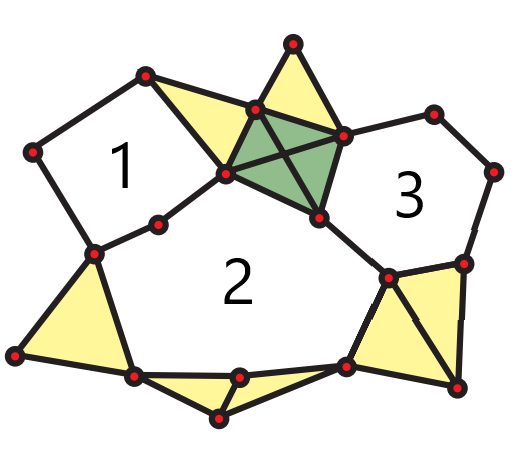
\includegraphics[width=.6\linewidth]{holes.png}
    \caption{\label{fig:holes} Example of a clique complex with three 1-dimensional holes (adapted from~\cite{ghrist:barcodes}).
    The number of these holes is equal to the first \emph{Betti number}.}
\end{figure}

%% Extracting features.
% Loop-back to main-story.
To extract these features using linear algebra, embed the clique complex into a Hilbert space $\mathcal{H}_k^G$, by raising the set of bitstrings that specify $(k+1)$-cliques to labels of orthonormal basis vectors.
Let $\mathcal{H}_k$ denote the Hilbert space spanned by computational basis states with Hamming weight\footnotemark[3] $k+1$.
Due to the way we encode cliques as bitstrings, we have that $\mathcal{H}_k^G$ is a subspace of  $\mathcal{H}_k$.
\footnotetext[3]{The Hamming weight of a bitstring is the number of 1s in it.}
Moreover, each $\mathcal{H}_k$ is an $\binom{n}{k+1}$-dimensional subspace of the entire $n$-qubit Hilbert space $\mathbb{C}^{2^n}$, and $\mathbb{C}^{2^n} \simeq \bigoplus_{k=-1}^{n-1}\mathcal{H}_k$.


% Detailed definition boundary maps (inc. restriction).
The next step towards extracting features using linear algebra involves studying properties of the \emph{boundary maps} $\partial_k :\mathcal{H}_k  \rightarrow \mathcal{H}_{k-1}$, which are defined by linearly extending the action on the basis states given by
\begin{align}
  \partial_k\ket{j} \coloneqq \sum_{i = 0}^{k}(-1)^i\ket{\widehat{j(i)}},
  \label{eq:boundary_map}
\end{align}
where $\widehat{j(i)}$ denotes the $n$-bit string of Hamming weight~$k$ that encodes the subset obtained by removing the $i$-th element from the subset encoded by $j$ (i.e., we set the $i$-th one in the bitstring $j$ to zero).
% Restriction of boundary maps
By considering the restriction of $\partial_k$ to $\mathcal{H}_k^G$ -- which we denote by~$\partial^G_k$ -- these boundary maps can encode the connectivities of the graph $G$, in which case their image and kernel encode various properties of the corresponding clique complex. 
% Intuition boundary maps.
Intuitively, these boundary maps map a $(k+1)$-clique to a superposition (i.e., a linear combination) of all $k$-cliques that it contains, as seen in Eq.~\eqref{eq:boundary_map}.

%% Homology groups.
These boundary maps allow one to extract features of the shape of a clique complex by studying their images and kernels, and in particular their quotients.
Specifically, the quotient space
\begin{align}
  H_k(G) \coloneqq \ker\partial_k^G /\Ima \partial_{k+1}^G,
  \label{eq:homology_group}
\end{align}
which is called the $k$-th \emph{homology group}, captures features of the shape of the underlying clique complex.
% Formal definition Betti numbers.
The main feature is the $k$-th \emph{Betti number} $\beta_k^G$, which is defined as the dimension of the $k$-th homology group, i.e., 
\[
\beta_k^G \coloneqq \dim H_k(G).
\]
% Intuition Betti numbers.
By construction, the $k$-th Betti number is equal to the number of $k$-dimensional holes in the clique complex.

%%% Betti numbers are central object in TDA.
The main problem in topological data analysis that we study in this paper is the computation of Betti numbers.
%% combinatorial Laplacians.
To do so, we study the \emph{combinatorial Laplacians}~\cite{eckmann:comb_lapl}, which are defined as
\begin{align}
\label{eq:comb_lapl}
\Delta_k^G= \left(\partial_k^G\right)^\dagger\partial^G_k + \partial_{k+1}^G\left(\partial_{k+1}^G\right)^\dagger.
\end{align}
% Intuition comb. Laplacian (i.e., generalization of ordinary graph Laplacian).
These combinatorial Laplacians can be viewed as generalized (or rather, higher-order) graph Laplacians in that they encode the connectivity between cliques in the graph as opposed to encoding the connectivity between individual vertices.
% Hodge theory -> Betti number computed as nullity of large sparse psd matrix.
We study the combinatorial Laplacians because the discrete version of the Hodge theorem~\cite{eckmann:comb_lapl} tells us that
\begin{align}
  \dim\ker\left(\Delta_k^G\right) = \beta_k^G,
  \label{eq:hodge}
\end{align}
which is often used as a more convenient way to compute Betti numbers~\cite{friedman:computing_betti}, particularly in the case of the quantum algorithm that we discuss in the next section.

% Wrapping back to example.
In conclusion, if the clique complex is constructed from a point cloud according to the construction discussed above, then computing these Betti numbers can be viewed as a method to extract features of the shape of the data (specifically, the number of holes are present at scale $\epsilon$).
% Varying scales epsilon.
By recording Betti numbers across varying scales $\epsilon$ in a so-called \emph{barcode}~\cite{ghrist:barcodes}, one can discern which holes are ``real'' and which are ``noise'', resulting in feature extraction that is robust to noise in the data.

% Figure w./ tda pipeline
\begin{figure*}
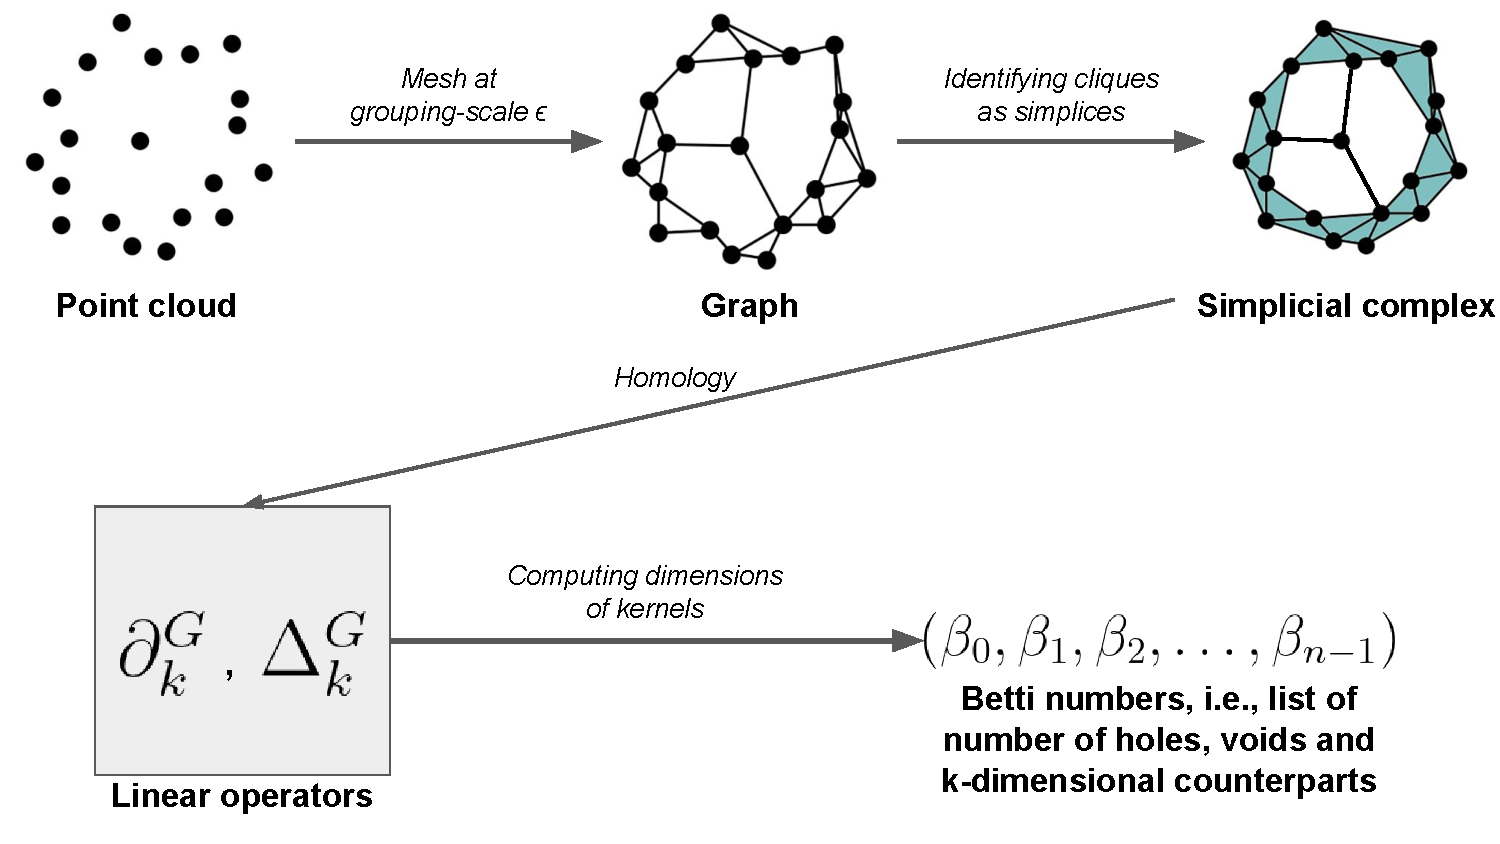
\includegraphics[width=0.825\textwidth]{pipeline}%
\centering
%\captionsetup{justification=centering}
\captionsetup{justification=raggedright}
\caption{\label{fig:tda} The pipeline of topological data analysis (adapted from~\cite{govek:figure}).
First, points that are within $\epsilon$ distance are connected to create a graph.
Afterwards, cliques in this graph are identified with simplices to create a simplicial complex.
Next, homology is used to construct linear operators that encode the topology.
Finally, the dimensions of the kernels of these operators are computed to obtain the Betti numbers which give the number of holes.}
\end{figure*}

%%%%%%%%%%%%%%%%%%%%%%%%%%%%%%%%%%%%%%%%%%%%%%%%%%
%%% Sec 2.2 (Quantum algorithm for BNE).
%%%%%%%%%%%%%%%%%%%%%%%%%%%%%%%%%%%%%%%%%%%%%%%%%%
\subsection{Quantum algorithm for Betti number estimation
\label{subsec:qalg_betti}}
\renewcommand{\thefootnote}{\fnsymbol{footnote}}
% TODO:
% - ...

%%% Introduction (inc. mention LGZ)
The algorithm for Betti number estimation of Lloyd, Garnerone and Zanardi (LGZ)~\cite{lloyd:lgz_algorithm} utilizes Hamiltonian simulation and phase estimation to estimate the dimension of the kernel (i.e., the \emph{nullity}) of the combinatorial Laplacian (which by Eq.~\eqref{eq:hodge} is equal to the corresponding Betti number).
%% Approach/ Idea: Hodge -> estimate nullity of comb. Lapl.
To make our presentation self-contained, we review this quantum algorithm for Betti number estimation (for a more in-depth review see~\cite{gunn:review}).

%%% Basic dea of the algorithm (SHUES).
% QPE + HS.
Estimating the nullity of a sparse Hermitian matrix can be achieved using some of the most fundamental quantum-algorithmic primitives. 
Namely, using Hamiltonian simulation and quantum phase estimation one can estimate the eigenvalues of the Hermitian matrix, given that the eigenvector register starts out in an eigenstate.
% Max mixed eigenvector register.
Moreover, if instead the eigenvector register starts out in the maximally mixed state (which can be thought of as a random choice of an eigenstate), then measurements of the eigenvalue register produce approximations of eigenvalues, sampled uniformly at random from the set of all eigenvalues.
% Repeat SUES to solve LLED.
This routine is then repeated to estimate the nullity by simply computing the frequency of zero eigenvalues (recall that the dimension of the kernel is equal to the multiplicity of the zero eigenvalue).
% LLED \neq NNUL.
Note that this procedure does not strictly speaking estimate the nullity, but rather the number of small eigenvalues, where the threshold is determined by the precision of the quantum phase estimation (see Section~\ref{subsubsec:approx_betti_numbers} for more details).
The steps of the quantum algorithm for Betti number estimation of LGZ are summarized in Figure~\ref{fig:lgz}.

\begin{figure}[h!]
{\hypersetup{citecolor=white}
  \begin{tcolorbox}[title=
    %
    {%\refstepcounter{figure}
       %Box \thefigure: 
       %\vspace{3pt}
       \hspace{-7pt}\mbox{Quantum algorithm for Betti number estimation}
       %\vspace{-7pt}
       %\label{fig:lgz}
       }]
\begin{enumerate}[leftmargin=*]
\item For $i = 1, \dots, M$ repeat:
  \begin{enumerate}[leftmargin=15pt]
  \item Prepare the state:
  \vspace{-5pt}
    \begin{align}
        \rho_k^G = \frac{1}{|\dim \mathcal{H}_k^G|}\sum_{j \in \text{Cl}_k(G)}\ket{j}\bra{j}.
        \label{eq:mixed_clique}
    \end{align}
  \vspace{-13pt}
  \item Apply quantum phase estimation to the unitary $e^{i\Delta_k^G}$, with the eigenvector register starting out in the state $\rho_k^G$.
  \item Measure the eigenvalue register to obtain an approximation $\widetilde{\lambda}_i$.
  \end{enumerate}
\item Output the frequency of zero eigenvalues:
\vspace{-5pt}
\begin{center}
    $\left|\{i \mid \widetilde{\lambda}_i = 0\}\right| / M$.
\end{center}
\end{enumerate}
\end{tcolorbox}
}

    \caption{Overview of the quantum algorithm of Lloyd, Garnerone and Zanardi (LGZ)~\cite{lloyd:lgz_algorithm}}
    \label{fig:lgz}
\end{figure}

\medskip 

%%% Analysis of steps of quantum algorithm for Betti number estimation.
%% Step 1a.
In Step~1(a), Grover's algorithm is used to prepare the uniform superposition over $\mathcal{H}_k^G$, from which one can prepare the state $\rho_k^G$ by applying a CNOT gate to each qubit of the uniform superposition into some ancilla qubits and tracing those out.
% Membership oracle / checking if bitstring encodes valid k-clique.
When given access to the adjacency matrix of $G$, one can check in $\bigO{k^2}$ operations whether a bitstring $j \in \{0, 1\}^n$ encodes a valid $k$-clique and mark them accordingly in the application of Grover's algorithm.
% Combinatorial numbersystem.
By cleverly encoding Hamming weight $k$ strings we can avoid searching over all $n$-bit strings, which requires $\bigO{nk}$ additional gates per round of Grover's algorithm plus an additional one-time cost of $\bigO{n^2k}$~\cite{gunn:review}.
% Runtime 1a.
Hence, the runtime of this first step is 
\[
\bigO{n^2k + nk^3\sqrt{\binom{n}{k+1}/\chi_k}} %= \bigO{n^2k + nk^3\sqrt{n^{k+1}/\chi_k}},
\]
where $\chi_k$ denotes the number of $(k+1)$-cliques. 
This runtime is polynomial in the number of vertices~$n$ when
\begin{align}
    \binom{n}{k+1}/\chi_k\in\bigO{\mathrm{poly}(n)}.
    \label{eq:clique_dense}
\end{align}

% Definition clique-dense.
Throughout this paper we say that a graph is \emph{clique-dense} if it satisfies Eq.~\eqref{eq:clique_dense}.
% Grover is actually not needed (i.e., rejection sampling).
Note that $\rho^G_k$ can of course also be directly prepared without the use of Grover's algorithm by using rejection sampling:\ choose a subset uniformly at random and accept it if it encodes a valid clique.
This is quadratically less efficient, however it has advantages if one has near-term implementations in mind, as it is a completely classical subroutine.
% Major bottleneck, see Sec~\ref{subsubsec:clique_density}
As we will discuss in more detail in Section~\ref{subsubsec:clique_density}, this state preparation procedure via Grover's algorithm or uniform clique-sampling is a crucial bottleneck in the quantum algorithm.

%% Step 1b.
% HS.
In Step~1(b), standard methods for Hamiltonian simulation of sparse Hermitian matrices are used together with quantum phase estimation to produce approximations of the eigenvalues of the simulated matrix.
% LGZ does B.
In the original algorithm, the matrix that LGZ simulates in this step is the \emph{Dirac operator}, which is defined as
\begin{align*}
  B_G = \begin{pmatrix}
    0 & \partial^G_1 & 0 & \dots & \dots & 0 \\
    \left(\partial^G_1\right)^\dagger & 0 & \partial^G_2 & \dots & \dots & 0\\
    0 & \left(\partial^G_2\right)^\dagger & 0 & \ddots & \dots & 0 \\
    \vdots & \vdots & \ddots & \ddots & \ddots & \vdots\\
    \vdots & \vdots & \vdots & \ddots&  0 & \partial^G_{n-1} \\
    0 & 0 & 0 & \dots & \left(\partial^G_{n-1}\right)^\dagger & 0 \\
  \end{pmatrix}
\end{align*}
and satisfies
\begin{align}
  B_G^2 =
  \begin{pmatrix}
    \Delta^G_0 & 0        & \dots & 0 \\
    0        & \Delta^G_2 & \dots & 0\\
    \vdots   & \vdots   & \ddots & 0 \\
    0        & 0        & \dots & \Delta^G_{n-1} \\
  \end{pmatrix}.
  \label{eq:dirac_lapl}
\end{align}

% B 'works'.
From Eq.~\eqref{eq:dirac_lapl} we gather that the probability of obtaining an approximation of an eigenvalue that is equal to zero is proportional to the nullity of the combinatorial Laplacian.
% Cost B.
Because $B_G$ is an $n$-sparse Hermitian matrix with entries $0, -1$ and $1$, to which we can implement sparse access using $\bigO{n}$ gates, we can implement $e^{iB}$ using $\bOt{n^2}$ gates~\cite{low:hs} (here $\widetilde{\mathcal{O}}$ suppresses logarithmically growing factors).


% Comb. Lapl directly also possible.
We remark that it is also possible to simulate $\Delta_k^G$ directly (as depicted in Figure~\ref{fig:lgz}).
% Cost Comb. Lapl.
Namely, as $\Delta_k^G$ is an $n^2$-sparse Hermitian matrix whose entries are bounded above by $n$, to which we can implement sparse access using $\bigO{n^4}$ gates (e.g., see Theorem 3.3.4~\cite{goldberg:comb_lapl}), we can implement $e^{i \Delta_k^G}$ using $\bOt{n^6}$ gates~\cite{low:hs}.

% Pros and cons.
The disadvantage to directly simulating $\Delta_k^G$ is that it requires more gates.
However, the advantage is that the Hamiltonian simulation of $\Delta_k^G$ requires fewer qubits compared to the Hamiltonian simulation of $B_G$, namely, $\log\binom{n}{k+1}$ qubits instead of $n$.
% Step can be replaced by sparse access to 'zero-padded' matrix.
Moreover, when the graph is clique-dense one can bypass Step~1(a) by padding $\Delta_k^G$ with all-zero rows and columns and letting the eigenvector start out in the maximally mixed state $I/2^n$ (see Section~\ref{subsubsec:reductions} for more details).

% Setup precision QPE (i.e., zero or not).
Let $\lambda_{\mathrm{max}}$ denote the largest eigenvalue and let $\lambda_{\mathrm{min}}$ denote the smallest nonzero eigenvalue of $\Delta_k^G$. 
By scaling down the matrix one chooses to simulate (i.e., either $B$ or $\Delta_k^G$) by $1/\lambda_{\mathrm{max}}$ to avoid multiples of $2\pi$, we can tell whether an eigenvalue is equal to zero or not if the precision of the quantum phase estimation is at least $\lambda_{\mathrm{max}}/ \lambda_{\mathrm{min}}$.
% Upper bound on lambda_max.
By the Gershgorin circle theorem (which states that $\lambda_{\mathrm{max}}$ is bounded above by the maximum sum of absolute values of the entries of a column or row) we know that $\lambda_{\mathrm{max}} \in \bigO{n}$. 
% No 'general' lower-bound on lambda_min.
For the general case not much is known in terms of lower bounds on $\lambda_{\mathrm{min}}$.
Nonetheless, even if we do not have such a lower bound, the number of small eigenvalues (as opposed to zero eigenvalues) still conveys topological information about the underlying graph (see Section~\ref{subsubsec:approx_betti_numbers} for more details).
% Runtime 1b.
By taking into account the cost of the quantum phase estimation~\cite{n&c}, the total runtime of Step~1(b) becomes~$\bOt{n^3/\lambda_{\mathrm{min}}}$.

%% Repetitions Step 1.
% eps-precision -> M = eps^{-2}.
Finally, estimating $\beta_k^G/\dim \mathcal{H}_k^G$ up to additive precision $\epsilon$ can be done using $M \in \bigO{\epsilon^{-2}}$ repetitions of Step~1(a) through 1(c).
% Total runtime quantum algorithm for Betti number estimation.
This brings the total cost of estimating $\beta_k^G/\dim \mathcal{H}_k^G$ up to additive precision~$\epsilon$ to
\begin{align*}
  \bOt{\left(nk^3\sqrt{\binom{n}{k+1}/\chi_k} + n^3/\lambda_{\mathrm{min}} \right)/\epsilon^2}.
  %\label{eq:runtime_lgz}
\end{align*}

%% qalg BNE efficient if smallest nonzero eigenvalue 1/poly and eff. max mixed.
In conclusion, the quantum algorithm for Betti number estimation runs in time polynomial in $n$ under two conditions.
Firstly, the graph has to be clique-dense, i.e., it has to satisfy Eq.~\eqref{eq:clique_dense} (see Section~\ref{subsubsec:clique_density} for more details).
Secondly, the smallest nonzero eigenvalue $\lambda_{\mathrm{min}}$ has to scale at least inverse polynomial in $n$ (see Section~\ref{subsubsec:approx_betti_numbers} for more details).
% -> superpoly speedup if both hold and |Cl_k(G)| = superpoly(n).
If both these conditions are satisfied, then the quantum algorithm for Betti number estimation achieves an exponential speedup over the best known classical algorithms if the size of the combinatorial Laplacian -- i.e., the number of $(k+1)$-cliques -- scales exponentially in $n$ (see Section~\ref{subsec:classical_algs} for more details). 

%%%%%%%%%%%%%%%%%%%%%%%%%%%%%%%%%%%%%%%%%%%%%%%%%%
%%% Sec 2.2.1 (Approximate Betti numbers).
%%%%%%%%%%%%%%%%%%%%%%%%%%%%%%%%%%%%%%%%%%%%%%%%%%
\subsubsection{Approximate Betti numbers
\label{subsubsec:approx_betti_numbers}}
% TODO:
% - ...

%% BNE vs (A)BNE.
% We cannot always solve BNE (i.e., unknown spectral gaps).
As mentioned in the previous section, the quantum algorithm for Betti number estimation does not strictly speaking estimate the Betti number (i.e., the nullity of the combinatorial Laplacian), but rather the number of small eigenvalues of the combinatorial Laplacian.
% Namely, spectral gap unknown.
This is because little is known in terms of lower bounds for the smallest nonzero eigenvalue of combinatorial Laplacians, and hence it is unclear to what precision one has to estimate the eigenvalues in the quantum phase estimation.
% Conjecture: inverse polynomial.
In any case, it is conjectured that for high-dimensional simplicial complexes the smallest nonzero eigenvalue is at least inverse polynomial in $n$~\cite{friedman:computing_betti}, which would imply that quantum phase estimation can in time $\bigO{\mathrm{poly}(n)}$ determine whether an eigenvalue is exactly equal to zero.

%% Nonetheless -> ABNE (!)
% However, we can still fix some precision (irregardless of spectral gap).
Even without knowing a lower bound on the smallest nonzero eigenvalue of the combinatorial Laplacian, we can still perform quantum phase estimation up to some fixed inverse polynomial precision.
% Output algorithm: number 'small' eigenvalues.
The quantum algorithm for Betti number estimation then outputs an estimate of the number of eigenvalues of the combinatorial Laplacian that lie below this precision threshold. 
% We call this: ABNE (as opposed to 'exact' Betti number estimation).
Throughout this paper we will refer to this as \emph{approximate Betti numbers}, which  turn out to still convey information about the underlying graph.
% Example: Cheeger's inequality.
For instance, Cheeger's inequality -- which relates the sparsest cut of a graph to the smallest nonzero eigenvalues of its standard graph Laplacian -- turns out to have a higher-order generalization that utilizes the combinatorial Laplacian~\cite{gundert:cheeger}.
Moreover, there are several other spectral properties of the combinatorial Laplacian beyond the number of small eigenvalues that also convey topological information about the underlying graph.
Some of these spectral properties can also be efficiently extracted using quantum algorithms (see Section~\ref{subsec:comb_lapl_beyond_betti} for more details).

%%%%%%%%%%%%%%%%%%%%%%%%%%%%%%%%%%%%%%%%%%%%%%%%%%
%%% Sec 2.2.2 (clique-density of graphs).
%%%%%%%%%%%%%%%%%%%%%%%%%%%%%%%%%%%%%%%%%%%%%%%%%%
\subsubsection{Efficient state preparation
  \label{subsubsec:clique_density}}
% TODO:
% - ...

%% Overview.
In Section~\ref{subsec:qalg_betti} we saw that the quantum algorithm for Betti number estimation can efficiently estimate approximate Betti numbers if the input graph satisfies certain criteria.
In particular, the graph has to be such that one can efficiently prepare the maximally mixed state over all its cliques of a given size (i.e., the state in Eq.~\eqref{eq:mixed_clique} in Figure~\ref{fig:lgz}).
In this section we highlight that this state preparation constitutes one of the main bottlenecks in the quantum algorithm for Betti number estimation.
%Ultimately, if we can efficiently sample a clique uniformly at random, then the quantum algorithm can efficiently estimate the corresponding approximate Betti number.

%% Max mixed via uniformly random clique sampling.
One way to prepare the maximally mixed state over all $k$-cliques of an $n$-vertex graph is to sample $k$-cliques uniformly at random and feed them into the quantum algorithm.
% Superpoly q-speedup if in time n^{o(k)}.
For the quantum algorithm for Betti number estimation to run in time sub-exponential in $n$, we have to be able to sample a $k$-clique uniformly at random in time $n^{o(k)}$.
However, for general graphs finding a $k$-clique cannot be done in time $n^{o(k)}$ unless the exponential time hypothesis fails~\cite{chen:clique}.
% Nonetheless, sometimes be eff.
Nonetheless, for certain families of graphs, uniform clique sampling can be done much more efficiently, e.g., in time polynomial in $n$ (in which case the quantum algorithm also runs in time polynomial in~$n$).
In particular, the graph's clique-density (i.e., probability that a uniformly random subset of vertices is a clique), or the graph's arboricity (which up to a factor $1/2$ is equivalent to the maximum average degree of a subgraph) are important factors that dictate the efficiency of uniform clique sampling algorithms.
In Section~\ref{subsec:graphs_quantum_advantage} we outline concrete families of graphs (based on their clique-density or arboricity) for which the quantum algorithm achieves a (superpolynomial) speedup over classical algorithms.

%%%%%%%%%%%%%%%%%%%%%%%%%%%%%%%%%%%%%%%%%%%%%%%%%%
%%% Sec 3 (Towards quantum advantage for BNE).
%%%%%%%%%%%%%%%%%%%%%%%%%%%%%%%%%%%%%%%%%%%%%%%%%%
\section{Towards quantum advantage for Betti number estimation
\label{sec:quantum_advantage}}
\renewcommand{\thefootnote}{\arabic{footnote}}
% TODO:
% - ...

%% Overview
In this section we discuss the advantages that the quantum algorithm for Betti number estimation can achieve over classical algorithms.
Firstly, in Section~\ref{subsec:prob_defs}, we precisely delineate and formally define the computational problems that the quantum algorithm for Betti number estimation can (efficiently) solve.
% Key steps can be applied beyond comb. Lapl.
In particular, it is clear that the techniques used in the quantum algorithm for Betti number estimation can also be used to estimate the number of small eigenvalues of arbitrary sparse Hermitian matrix, not just of combinatorial Laplacians.
% -> llsd, the natural generalization.
We take this as the starting point to define our natural generalization, which is called \emph{low-lying spectral density} estimation (a version of which was also studied by Brand\~{a}o~\cite{brandao:thesis}).
% DQC1-hardness.
Next, in Section~\ref{subsec:hardness_lled}, we show that this generalization is $\mathsf{DQC1}$-hard, which suggests that the quantum-algorithmic methods behind the quantum algorithm for Betti number estimation may be a source of exponential separation between quantum and classical computers.
We also discuss how to potentially close the gap between the topological data analysis problem of Betti number estimation and its generalization, which would show that the topological data analysis problem is itself classically intractable.
%% Beyond complexity theory / state-of-the-art classical algorithms.
Setting aside the complexity theory, in Section~\ref{subsec:classical_algs} we discuss the state-of-the-art classical algorithms for Betti number estimation and compare them with the quantum algorithms for Betti number estimation.
We also discuss promising approaches for developing novel more efficient classical algorithms that take into account the specifics of the combinatorial Laplacian and we clearly delineate the theoretical hurdles that, at least currently, stymie such classical approaches.
% Graphs with quantum advantage
After discussing the strengths and weaknesses of the classical algorithms, we identify graphs for which the quantum algorithm can achieve (superpolynomial) speedups over the best known classical algorithms in Section~\ref{subsec:graphs_quantum_advantage}.
%%%%%%%%%%%%%%%%%%%%%%%%%%%%%%%%%%%%%%%%%%%%%%%%%%
%%% Sec 3.1 (Problem definitions).
%%%%%%%%%%%%%%%%%%%%%%%%%%%%%%%%%%%%%%%%%%%%%%%%%%
\subsection{Problem definitions
\label{subsec:prob_defs}}
% TODO:
% - ...

%% In this section: we formally define problems we study.
In this section we formally define the computational problems whose hardness we will study.
%% Key steps of LGZ.
We begin by defining the problems that capture the key steps of the quantum algorithm for Betti number estimation.
%% Problems solved by LGZ.
Afterwards, we define the problems related to topological data analysis that the quantum algorithm for Betti number estimation aims to solve.
% 3/4. BNE & ABNE.
%That is, we define the problems of Betti number and approximate Betti number estimation.
% 4. End section: reductions.
We end this section by discussing the precise relationships between these problems.

%%% General background.
The input matrices that we consider are sparse positive semidefinite matrices.
%% We define problems for sparse psd matrices.
We call a $2^n \times 2^n$ positive semidefinite matrix $\emph{sparse}$ if at most $\bigO{\mathrm{poly}(n)}$ entries in each row are nonzero.
% Definition log-local
A special class of sparse positive semidefinite matrices that we consider is the class of \emph{log-local} Hamiltonians, i.e., $n$-qubit Hamiltonians that can be written as a sum
\begin{align}
  H = \sum_{j=1}^m H_j,
  \label{eq:local_terms}
\end{align}
where each $H_j$ acts on at most $\bigO{\log n}$ qubits and we assume that $m\in\bigO{\mathrm{poly}(n)}$.

%%% Input models.
Our problems take as input a specification of a sparse positive semidefinite matrix, and we consider the following two standard cases.
%% 1. Sparse access.
First, we consider the case where the input matrix is specified in terms of \emph{sparse access}.
% Intuition operation of the oracle/circuit.
That is, the input matrix $H \in \mathbb{C}^{2^n \times 2^n}$ is specified by quantum circuits that let us query the values of its entries, and the locations of the nonzero entries.
% Formal definition of the oracle/circuit.
More precisely, we assume that we are given classical descriptions of $\bigO{\mathrm{poly}(n)}$-sized quantum circuits that implement the oracles $O_H$ and $O_{H, \mathrm{loc}}$, which map
\begin{align*}
  O_H&: \ket{i, j}\ket{0} \mapsto \ket{i, j}\ket{H_{i,j}},\\
  O_{H, \mathrm{loc}}&: \ket{j, \ell}\ket{0} \mapsto \ket{j, \ell}\ket{\nu(j, \ell)},
\end{align*}
where $0 \leq i, j , \ell \leq 2^n - 1$, and $\nu(j, \ell) \in \{0, \dots, 2^n - 1\}$ denotes the location of the $\ell$-th nonzero entry of the $j$-th column of~$H$.
%% 2. Local terms.
Secondly, for log-local Hamiltonians, we also consider specifying the input matrix $H$ by its \emph{local-terms} $\{H_j\}$ as in Eq.~\eqref{eq:local_terms}.

%%% Intro of 'approx sampling'.
In order to define the problem of generating approximations of eigenvalues that are sampled uniformly at random, we fix a suitable notion of an approximation of a probability distribution.
In particular, this notion needs to take into account that the algorithm may err on both the estimation of the eigenvalue, and on the probability with which it provides such an estimation.
% Source of definition
For this we use the following definition presented in~\cite{wocjan:bqp_complete}.
% Definition of 'approx sampling'.
Let $p$ be some probability distribution over the eigenvalues of a positive semidefinite matrix $H \in \mathbb{C}^{2^n \times 2^n}$.
That is, sampling according to $p$ will output an eigenvalue $\lambda_k$ with probability $p(\lambda_k)$, and $\sum_{k=0}^{2^n -1}p(\lambda_k) = 1$. 
In this context, a probability distribution $q$ with finite support $Y_q \subset \mathbb{R}$ is said to be an \emph{$(\delta, \mu)$-approximation} of $p$ if it satisfies
\[
  \sum_{y \in Y_q\text{ }:\text{ }|y - \lambda_k| < \delta}q(y) \geq (1-\mu)p(\lambda_k),\enskip \forall k \in \{0, \dots, 2^{n-1}\}.
\]
% Intuition behind definition 'approx sampling'.
Intuitively, this means that if we draw a sample according to $q$, then this sample will be $\delta$-close to an eigenvalue $\lambda_k$ with probability at least $(1-\mu)p(\lambda_k)$\footnotemark[1].\footnotetext[1]{This definition captures the distribution generated by quantum phase estimation:\ the eigenvector is chosen according to the distribution $p$ specified by the input state, and the output is $\delta$-close to the corresponding eigenvalue with probability at least $(1-\mu)$.}
%%% Formal problem definition SUES.
Using this definition, we define the problem of generating approximations of eigenvalues that are sampled uniformly at random from the set of all eigenvalues as follows.

% Definition SUES
\vspace{5pt}
\noindent\begin{tabularx}{\linewidth}{l X c}
  \multicolumn{2}{l}{\textbf{\textsf{Sparse uniform eigenvalue sampling (SUES)}}\footnotemark[2]} \\
  \multicolumn{2}{l}{\textbf{Input:}} \\
  1) & A sparse positive semidefinite matrix $H\in\mathbb{C}^{2^n \times 2^n}$, with $||H|| \leq \mathrm{poly}(n)$.\\
  2) & An estimation precision $\delta \in \Omega\left(1/\mathrm{poly}(n)\right)$.\\
  3) & An error probability $\mu \in \Omega\left( 1/\mathrm{poly}(n)\right)$.
\end{tabularx}
\noindent\begin{tabularx}{\linewidth}{l X c}
  \textbf{Output:} & A sample drawn according to a $(\delta, \mu)$-approximation of the uniform distribution over the eigenvalues of $H$.
\end{tabularx}
\footnotetext[2]{In view of noisy quantum computers, it is interesting to consider distributions that are close to these $(\delta,\mu)$-approximation in total variation distance.
Sampling such distributions can be less demanding, however, the precise hardness remains to be analyzed.}

%%% Introduction llsd.
% SUES used for 'fraction small eigenvalues' in qalg for Betti number estimation.
In the quantum algorithm for Betti number estimation, samples from \textsc{sues} are used to estimate the number of eigenvalues of the combinatorial Laplacian that are close to zero.
% Can go beyond comb. Lapl.
Clearly, this same idea can be used to estimate the number of eigenvalues that lie in some given interval for arbitrary sparse positive semidefinite matrices.
% Formal definition eigenvalue count (i.e., 'fraction eigenvalues in interval').
This is called the \emph{eigenvalue count}~\cite{brandao:thesis}, which for a positive semidefinite matrix $H~\in~\mathbb{C}^{2^n \times 2^n}$ and eigenvalue thresholds $a, b \in \mathbb{R}_{\geq 0}$ is given by
\begin{align*}
  N_H(a, b) = \frac{1}{2^n}\sum_{k\text{ }:\text{ }a \leq \lambda_k\leq b}1,
\end{align*}
where $\lambda_0 \leq \dots \leq \lambda_{2^n-1}$ denote the eigenvalues of $H$.
% -> Fraction small eigenvalue N_H(0, threshold).
For a threshold $b \in \Omega\left(1/\mathrm{poly}(n)\right)$, we shall refer to the quantity $N_H(0, b)$ as \emph{low-lying spectral density}.
This precisely captures our notion of the number of eigenvalues close to zero as discussed before.
%%% Formal problem definition llsd.
We define the problem of estimating the low-lying spectral density as follows.

% Definition llsd
\vspace{3pt}
\noindent\begin{tabularx}{\linewidth}{l X c}
  \multicolumn{2}{l}{\textbf{\textsf{Low-lying spectral density estimation (LLSD)}}\footnotemark[3]} \\
  \multicolumn{2}{l}{\textbf{Input:}}\\
  1) & A sparse positive semidefinite matrix $H \in \mathbb{C}^{2^n \times 2^n}$, with $||H|| \leq \mathrm{poly}(n)$.\\
  2) & A threshold $b \in \Omega\left(1/\mathrm{poly}(n)\right)$.\\
  3) & Precision parameters $\delta, \epsilon \in \Omega\left(1/\mathrm{poly}(n)\right)$.\\
  4) & A success probability $\mu > 1/2$.\\
\end{tabularx}
\noindent\begin{tabularx}{\linewidth}{l X c}
  \textbf{Output:} & An estimate $\chi \in [0,1]$ that, with probability at least $\mu$, satisfies
\end{tabularx}
\vspace{-3pt}
\begin{align*}
    N_H\left(0, b\right) - \epsilon \leq \chi \leq N_H(0, b + \delta) + \epsilon.
\end{align*}

% Ref to Brown et al.
\footnotetext[3]{The exact version of this problem is closely related to $\mathsf{\# P}$~\cite{brown:dos}.}

%%% Idea llsd: repeatedly sample SUES and output frequency of 'small eigenvals'.
To provide some intuition behind this definition, note that it is supposed to precisely capture the problem that is solved by repeatedly sampling from \textsc{sues} and computing the frequency of the eigenvalues that lie below the given threshold.
% Delta due to 'QPE precision'.
We therefore require the precision parameter~$\delta$ due to the imprecisions in the quantum phase estimation algorithm.
% Epsilon due to 'sampling error'.
Moreover, the precision parameter~$\epsilon$ is necessary due to the sampling error we incur by estimating a probability by a relative frequency.

%%% Introduction BNE. 
% Motivation: TDA problems that above allows us to solve.
Now that we have formally defined the problems that capture the key steps of the quantum algorithm for Betti number estimation, we define the problems related to topological data analysis that they allow us to solve.
% Input is the graph, not the comb. Lapl.
For these problems we consider the adjacency matrix of the graph to be the input, as this is usually the input to the quantum algorithm for Betti number estimation.
%%% Formal problem definition BNE.
We define the problem of estimating Betti numbers as follows.

% Definition BNE
\vspace{5pt}
\noindent\begin{tabularx}{\linewidth}{l X c}
  \multicolumn{2}{l}{\textbf{\textsf{Betti number estimation (BNE)}}\footnotemark[4]} \\
  \multicolumn{2}{l}{\textbf{Input:}}\\
  1) & The adjacency matrix of a graph $G = ([n], E)$.\\
  2) & An integer $0 \leq k \leq n-1.$\\
  3) & A precision parameter $\epsilon \in \Omega\left(1/\mathrm{poly}(n)\right)$.\\
  4) & A success probability $\mu > 1/2$.\\
\end{tabularx}
\noindent\begin{tabularx}{\linewidth}{l X c}
  \textbf{Output:} & An estimate $\chi \in [0,1]$ that, with probability at least $\mu$, satisfies
\end{tabularx}
\vspace{-3pt}
\begin{align*}
   \left|\chi - \frac{\beta_k^G}{\dim \mathcal{H}_k^G}\right| \leq \epsilon.
\end{align*}

% Ref to Brown et al.
\footnotetext[4]{The exact version of this problem is $\mathsf{NP}$-hard~\cite{adamaszek:betti_np}}

%%% Introduction ABNE.
% Qalg Betti number estimation only solves BNE in certain regimes.
As discussed in Section~\ref{subsubsec:approx_betti_numbers}, the quantum algorithm for Betti number estimation does not precisely solve the above problem.
% Namely, smallest nonzero eigenvalue has to be 1/poly.
Namely, due to the lack of knowledge regarding lower bounds on the smallest nonzero eigenvalue of the combinatorial Laplacian, we are not always able to estimate the number of eigenvalues that are exactly equal to zero.
% However, if not qalg for Betti number still estimates so-called 'approximate Betti numbers'.
Nonetheless, the quantum algorithm for Betti number estimation is still able to estimate the number of eigenvalues of the combinatorial Laplacian that are close to zero, which we called approximate Betti numbers.
%%% Formal problem definition ABNE.
We define the problem of estimating approximate Betti numbers as follows.

% Definition ABNE
\vspace{5pt}
\noindent\begin{tabularx}{\linewidth}{l X c}
  \multicolumn{2}{l}{\textbf{\textsf{Approximate Betti number estimation (ABNE)}}} \\
  \multicolumn{2}{l}{\textbf{Input:}}\\
  1) & The adjacency matrix of a graph $G = ([n], E)$.\\
  2) & An integer $0 \leq k \leq n-1.$\\
  3) & Precision parameters $\delta, \epsilon \in \Omega\left(1/\mathrm{poly}(n)\right)$.\\
  4) & A success probability $\mu > 1/2$.\\
\end{tabularx}
\noindent\begin{tabularx}{\linewidth}{l X c}
  \textbf{Output:} & An estimate $\chi \in [0,1]$ that, with probability at least $\mu$, satisfies
\end{tabularx}
\vspace{-3pt}
\begin{align*}
    \frac{\beta_k^G}{\dim \mathcal{H}_k^G} - \epsilon \leq \chi \leq N_{\Delta_k^G}(0, \delta) + \epsilon.
\end{align*}

%%% "Problem solved by LGZ".
We are now set to outline the problem that the quantum algorithm for Betti number estimation can efficiently solve.
% Qalg Betti number estimation only solves ABNE in certain regimes.
As discussed in Section~\ref{subsubsec:clique_density}, the quantum algorithm for Betti number estimation can efficiently solve \textsc{abne}, but only in certain regimes.
% Namely, efficient sparse access Delta_k^G or preparation max. mixed states H_k^G.
In particular, one has to be able to efficiently prepare the maximally mixed state over all cliques of a given size from the adjacency matrix of the graph.
% Sufficient condition (i): clique-dense (as done in qalg Betti number estimation)!
As mentioned in Section~\ref{subsubsec:clique_density}, the efficiency of this state preparation depends on the graph's clique-density (i.e., probability that a uniformly random subset of vertices is a clique), or the graph's arboricity (which up to a factor $1/2$ is equivalent to the maximum average degree of a subgraph).
% Conclusion: LGZ solves ABNE in clique-dense regime.
In short, the problem that the quantum algorithm for Betti number estimation can efficiently solve is a restriction of \textsc{abne}, where one is promised that the input graph is such that one can efficiently prepare the maximally mixed state over all cliques of a given size from the adjacency matrix (e.g., if the graph is sufficiently clique-dense or if it has a sufficiently bounded arboricity).
We discuss this in more detail in Section~\ref{subsec:graphs_quantum_advantage}, where we outline sufficient conditions on the graph's clique-density or arboricity that allow the quantum algorithm to efficiently solve \textsc{abne}. 

%%% Discussion (llsd is really generalization of ABNE)
Next, we will study the complexity of \textsc{llsd} as it is a generalization of the problem that the quantum algorithm for Betti number estimation efficiently solves.
% Meaning: llsd restricted to comb. Lapl. is equivalent to abne.
Namely, as we will show in the following section, we can use \textsc{llsd} to directly solve the problem that the quantum algorithm for Betti number estimation efficiently solves.
% ABNE has different input
Note that the input to the quantum algorithm for Betti number estimation is the adjacency matrix, and not the combinatorial Laplacian.
Therefore, in order to use \textsc{llsd} to solve the problem that the quantum algorithm for Betti number estimation efficiently solves, one first has to construct the appropriate input to \textsc{llsd}.
% Directly comb. Lapl. too expensive.
As it is computationally too expensive to enumerate all cliques in your graph, we cannot take the straightforward approach of first computing the combinatorial Laplacian to construct the desired input to \textsc{llsd}. 
% Fortunately, also other option.
Fortunately, we can still use \textsc{llsd} to efficiently solve the problem that the quantum algorithm for Betti number estimation efficiently solves by simulating sparse access to a matrix that is obtained by padding the combinatorial Laplacian with all-zeros columns and rows (see Section~\ref{subsubsec:reductions} for more details).
% LGZ circumvent with rho_k^G.
%Note that in the quantum algorithm for Betti number estimation this is achieved by first preparing the maximally mixed state over $\mathcal{H}_k^G$.

%%%%%%%%%%%%%%%%%%%%%%%%%%%%%%%%%%%%%%%%%%%%%%%%%%
%%% Sec 3.1.1 (Relationships between the problems).
%%%%%%%%%%%%%%%%%%%%%%%%%%%%%%%%%%%%%%%%%%%%%%%%%%
\subsubsection{Relationships between the problems
\label{subsubsec:reductions}}
% TODO:
% - ...

%% Purpose of section: formally elucidate relations problems defined in previous section.
In the previous section we have formally defined the computational problems whose complexity we will study.
In this section we examine the reductions between \textsc{llsd} and the problems related to topological data analysis in order to elucidate the precise relationships.
% Overview in fig:reductions.
An overview of the reductions can be found in Figure~\ref{fig:reductions}.

%%% llsd vs ABNE
First, we discuss the relationship between \textsc{llsd} and \textsc{abne}.
%% 2. llsd \approx ABNE, if H = comb. Lapl.
It is clear that \textsc{llsd} with a combinatorial Laplacian as input produces a solution to the corresponding instance of \textsc{abne}.
%% 3. ABNE <= llsd, if eff. sparse access or preperation max. mixed state.
It is also clear that \textsc{llsd} can be used to solve \textsc{abne} if given the input of \textsc{abne} (i.e, the adjacency matrix), we can efficiently implement sparse access to a matrix such that an estimate of its low-lying spectral density allows us to recover an estimate of the low-lying spectral density of the combinatorial Laplacian.
% Example of when sparse access / max. mixed state: clique-dense.
Interestingly, it turns out that we can do so if the input graph is clique-dense (i.e., in precisely the regime that is efficiently solvable by the quantum algorithm for Betti number estimation).
% Max mixed as in qalg for Betti number estimation.
Namely, we can efficiently implement sparse access to the $\binom{n}{k+1} \times \binom{n}{k+1}$-sized matrix $\Gamma_k^G$ whose columns and rows are indexed by $(k+1)$-subsets of vertices, and whose entries are given by
\begin{align}
  \left(\Gamma_k^G\right)_{i, j} =
  \begin{cases} (\Delta_k^G)_{i, j} & \text{if $i$ and $j$ are $(k+1)$-cliques,}\\ 0 & \text{otherwise}.
  \end{cases}
\label{eq:gamma_matrix}
\end{align}
In other words, the entries of the columns and rows that correspond to $(k+1)$-cliques are equal to the corresponding entries of the combinatorial Laplacian, and all other entries are equal to zero.
After subtracting the extra nullity caused by adding the $\binom{n}{k+1} - \chi_k$ all-zeros columns and rows, and renormalizing the eigenvalue count by a factor $\binom{n}{k+1}/\chi_k$, the low-lying spectral density of this $\Gamma_k^G$ is equal to the low-lying spectral density of the combinatorial Laplacian.
In equation form, we have that
\begin{align}
  N_{\Delta_k^G}(0, b) = \frac{\binom{n}{k+1}}{\chi_k}N_{\Gamma_k^G}(0, b) - \frac{\binom{n}{k+1} - \chi_k}{\chi_k}.
  \label{eq:llsd_delta_gamma}
\end{align}
From Eq.~\eqref{eq:llsd_delta_gamma}, it is clear that an estimate of $N_{\Gamma_k^G}(0, b)$ up to additive inverse polynomial precision allows us to obtain an estimate of $N_{\Delta_k^G}(0, b)$ up to additive inverse polynomial precision, assuming indeed that the graph is clique-dense -- i.e., that $\chi_k/\binom{n}{k+1} \in \Omega\left(1/\mathrm{poly}(n)\right)$.
Note that this also requires us to have an estimate of $\chi_k/\binom{n}{k+1}$.
Since the graph is clique-dense, it suffices to estimate $\chi_k/\binom{n}{k+1}$ up to additive inverse polynomial precision.
An estimate of $\chi_k/\binom{n}{k+1}$ up to additive error $\epsilon$ can be obtained by drawing $\mathcal{O}(\epsilon^{-2})$ many $k$-subsets of vertices uniformly at random, and computing the fraction of these subsets that constitute an actual $k$-clique.

%% Observation: ABNE <= llsd precisely when LGZ can eff solve ABNE.
We emphasize that the above reduction works in precisely the regime where the quantum algorithm for Betti number estimation can efficiently solve \textsc{abne}.
In other words, \textsc{llsd} can be used to directly solve the problem that the quantum algorithm for Betti number estimation can efficiently solve.
% => llsd strict generalization of problem solved by quantum algorithm for Betti number estimation.
In this regard, \textsc{llsd} is indeed a generalization of the problem that the quantum algorithm for Betti number estimation can efficiently solve.

%% 4. ABNE vs BNE
Finally, let us discuss the reductions between \textsc{abne} and \textsc{bne}.
% BNE <= ABNE , if smallest nonzero eigenvalue is at least 1/poly.
It is clear that \textsc{bne} is reducible to \textsc{abne} if the size of the smallest nonzero eigenvalue of the combinatorial Laplacian is at least inverse polynomial in $n$.
% ABNE <= BNE, unclear (llsd vs NNull).
The reverse direction is unclear, as for \textsc{bne} the threshold on the eigenvalues is fixed to be exactly zero.
% Possible approach: projecting eigenvalues below b to zero.
A possible approach would be to first project the eigenvalues that lie below the given threshold to zero and then count the zero eigenvalues.
However, using techniques inspired by ideas from~\cite{gilyen:block, kitaev:book}, we have only been able to project these eigenvalues close to zero, as opposed to exactly equal to zero, and we are not aware of any way to circumvent this.

% Figure w./ summary of reductions
\begin{figure*}
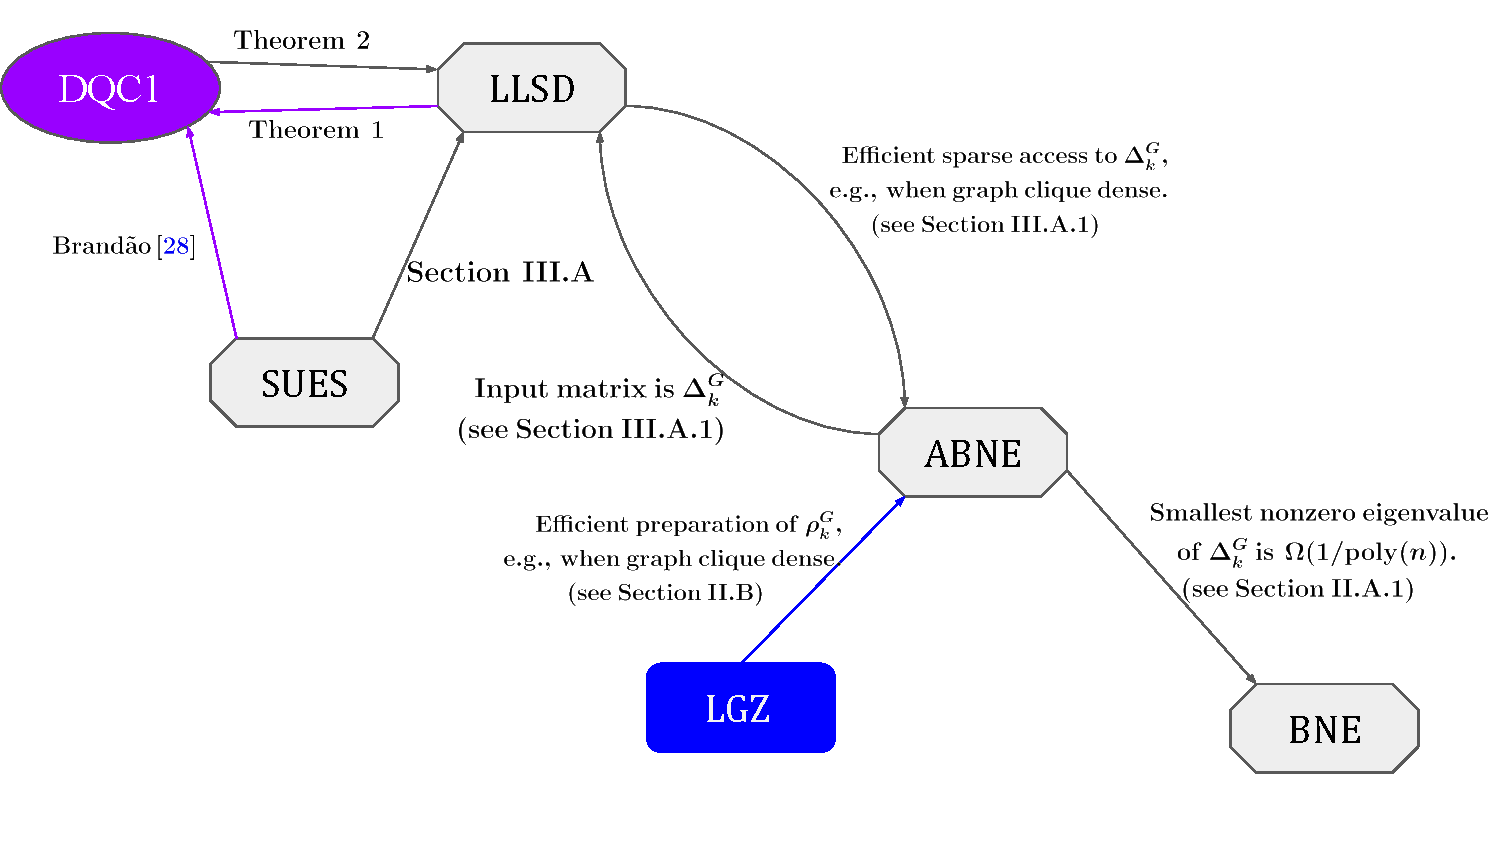
\includegraphics[width=0.9\textwidth]{diagram}%
\captionsetup{justification=raggedright}
\caption{\label{fig:reductions} Overview of the relations between the problems (octagons), algorithm (rectangle) and complexity class (ellipse) studied in this paper. 
A $\stackrel{\rm C}{\longrightarrow}$ B stand for:\ ``A can efficiently solve B if condition C holds''.
The algorithm studied is that by Lloyd, Garnerone and Zanardi (LGZ) as described in Figure~\ref{fig:lgz}.
The problems are sparse uniform eigenvalue sampling (\textsc{sues}), low-lying spectral density estimation (\textsc{llsd}), approximate Betti number estimation (\textsc{abne}), and Betti number estimation (\textsc{bne}) as defined in Section~\ref{subsec:prob_defs}
The class $\mathsf{DQC1}$ is defined in Section~\ref{subsubsec:dqc1}.}
\end{figure*}

%%%%%%%%%%%%%%%%%%%%%%%%%%%%%%%%%%%%%%%%%%%%%%%%%%
%%% Sec 3.2 (Classical hardness of LLED).
%%%%%%%%%%%%%%%%%%%%%%%%%%%%%%%%%%%%%%%%%%%%%%%%%%
\subsection{Classical intractability of low-lying spectral density estimation}
\label{subsec:hardness_lled}
% TODO:
% - ...

% Holy grail.
To show that quantum computers have an advantage over classical computers in topological data analysis, one would have to show that Betti number estimation requires exponential time on a classical computer.
% This section.
In this section we study the classical hardness of the problem efficiently solved by the quantum algorithm for Betti number estimation.
In particular, we show that the natural generalization of this problem (which we called low-lying spectral density estimation) is classically intractable under widely-believed complexity-theoretic assumptions by showing that it is hard for the one clean qubit model of computation.
% Close the gap.
Afterwards, we discuss how to potentially close the gap between the classical intractability of low-lying spectral density and (approximate) Betti number estimation in order to show that the topological data analysis problem is itself classically intractable. 

%%%%%%%%%%%%%%%%%%%%%%%%%%%%%%%%%%%%%%%%%%%%%%%%%%
%%% Sec 3.2.1 (The one clean qubit model).
%%%%%%%%%%%%%%%%%%%%%%%%%%%%%%%%%%%%%%%%%%%%%%%%%%
\subsubsection{The one clean qubit model of computation}
\label{subsubsec:dqc1}
% TODO:
% - ...

%% Motivate DQC1 (closely related to complexity problems in previous section).
In the next section we will show that the complexity of the problems defined in Section~\ref{subsec:prob_defs} are closely related to the one clean qubit model of quantum computation~\cite{knill:dqc1}.
% Definition $\mathsf{DQC1}$.
In this model we are given a quantum register that is initialized in a state consisting of a single `clean' qubit in the state $\ket{0}$, and $n-1$ qubits in the maximally mixed state.
We can then apply any polynomially-sized quantum circuit to this register, and measure only the first qubit in the computational basis.
Following~\cite{knill:dqc1}, we will refer to the complexity class of problems that can be solved in polynomial time using this model of computation as $\mathsf{DQC1}$ -- ``deterministic quantum computation with a single clean qubit''.

%% Formal definition DQC1-hardness (poly-time truth-table reductions).
We will refer to a problem as $\mathsf{DQC1}$-hard if any problem in $\mathsf{DQC1}$ can be reduced to it under polynomial time truth-table reductions.
% Explanation 'poly-time truth-table reduction'.
That is, a problem $L$ is $\mathsf{DQC1}$-hard if we can solve any problem in $\mathsf{DQC1}$ using polynomially many nonadaptive queries to an oracle for $L$, together with polynomial time preprocessing of the inputs and postprocessing of the outcomes.
%% Decision vs estimation.
Technically, instead of containing the problem of estimating a given quantity up to additive inverse polynomial precision, $\mathsf{DQC1}$ contains the decision problem of deciding whether this quantity is greater than $1/2 + \sigma$ or less than $1/2 - \sigma$, where $\sigma$ is some inverse polynomial gap.
% WLOG, we can focus on estimation.
However, as the estimation versions of these problems are straightforwardly reduced to their decision version using binary search, we will bypass this point from now on and only consider the problems of estimating a given quantity up to inverse polynomial precision~\cite{shor:dqc1}.

%% DQC1 beyond classical (inc. -> DQC1-hard classically intractable).
It is widely believed that the one clean qubit model of computation is more powerful than classical computation.
% Complete problems seem hard.
For instance, estimating quantities that are supposedly hard to estimate classically, such as the normalized trace of a unitary matrix corresponding to a polynomial-depth quantum circuit and the evaluation of a Jones polynomial at a root of unity, turn out to be complete problems for $\mathsf{DQC1}$~\cite{shor:dqc1}.
% Sampling from output impossible (under some complexity theoretical conjectures).
Moreover, it has been shown that classical computers cannot efficiently sample from the output distribution of the one clean qubit model up to constant total variation distance error, provided that some complexity theoretic conjectures hold~\cite{tomoyuki:dqc1, tomoyuki:dqc1_k}.

%%%%%%%%%%%%%%%%%%%%%%%%%%%%%%%%%%%%%%%%%%%%%%%%%%
%%% Sec 3.2.2 (DQC1-hardness of LLED).
%%%%%%%%%%%%%%%%%%%%%%%%%%%%%%%%%%%%%%%%%%%%%%%%%%
\subsubsection{Hardness of low-lying spectral density estimation for the one clean qubit model
\label{subsec:results}}
% TODO:
% - ...

%%% Battleplan/goal: hardness of problem solved by LGZ.
Recall that in order to show that quantum computers have an advantage over classical computers in topological data analysis, one would have to show that the problem that the quantum algorithm for Betti number estimation can efficiently solve is hard for classical computers.
% Problem solved by LGZ <-> ABNE in certain regimes.
In Section~\ref{subsec:prob_defs}, we pointed out that the problem that the quantum algorithm for Betti number estimation can efficiently solve is a restriction of \textsc{abne} to clique-dense graphs (i.e., graphs which satisfy Eq.~\eqref{eq:clique_dense}).
% In this regime: llsd strict generalization of LGZ
Moreover, we showed in Section~\ref{subsubsec:reductions} that \textsc{llsd} is a generalization of this version of \textsc{abne}.
% Motivates us to look at hardness of llsd.
This motivates us to study the classical hardness of \textsc{llsd}.
% Main result: DQC1-hardness of the generalization llsd.
In this section we present our results, which show that the complexity of \textsc{llsd} is intimately related to the one clean qubit model.

% First / most important result: hardness.
Our first and main result is that \textsc{llsd} is hard for the class $\mathsf{DQC1}$, even when the input is restricted to log-local Hamiltonians.
% DQC1-hard -> Classically hard.
As the one clean qubit model of computation is widely believed to be more powerful than classical computation, this shows that \textsc{llsd} is likely hard for classical computers.
% More in next section.
We discuss the implications of this result on the classical hardness of the problem that the quantum algorithm for Betti number estimation can efficiently solve in Section~\ref{subsubsec:discussion}.

% Theorem: $\mathsf{DQC1}$-hardness of llsd.
\begin{theorem}
  \textsc{llsd} is $\mathsf{DQC1}$-hard.
  Moreover, \textsc{llsd} with the input restricted to log-local Hamiltonians remains $\mathsf{DQC1}$-hard.
 \label{thm:dqc1_hardness_llsd}
\end{theorem}

%% Proof-sketch.
We now give a sketch of our proof of the above theorem, the complete proof can be found in the Supplemental Material.
% Reduction to kind of (normalized) subtrace.
The main idea behind the proof is to show that we can use \textsc{llsd} to estimate a quantity similar to a normalized subtrace -- or more precisely, a normalized sum of eigenvalues below a given threshold -- which has been shown to be $\mathsf{DQC1}$-hard by Brand\~{a}o~\cite{brandao:thesis}.
% Approach: bin approx of spectrum and compute area under it.
We estimate this normalized subtrace by constructing a histogram approximation of the low-lying eigenvalues, and afterwards computing the mean of this histogram.
To construct this histogram, we use \textsc{llsd} to estimate the number of eigenvalues that lie in each bin.
% Double counting due to imprecisions around thresholds.
To avoid double counting of eigenvalues due to imprecisions around the thresholds of the bins, we subtract the output of \textsc{llsd} with the eigenvalue threshold set to the lower-threshold of the bin from the output of \textsc{llsd} with the eigenvalue threshold set to the upper-threshold of the bin. 
By doing so, we obtain an estimate of the number of eigenvalues within the bin, and misplace eigenvalues by at most one bin\footnotemark[1].
\footnotetext[1]{
  We believe that our approach could be modified to a Karp reduction by encoding an instance of the normalized subtrace estimation problem into a single instance of \textsc{llsd}.
  This would entail manipulating the Kitaev circuit-to-Hamiltonian construction and taking direct sums of matrices.
  As this reduction is not vital for our claim, we leave this question open for future work.}

%%% Introduction upper bounds.
Our second result shows that the complexity of \textsc{llsd} is more closely related to $\mathsf{DQC1}$ than just hardness.
Namely, we point out that if the input to \textsc{llsd} is restricted to log-local Hamiltonians (or more generally, any type of Hamiltonian that allows for efficient Hamiltonian simulation using $\bigO{\log(n)}$ ancilla qubits), then it can be solved using the one-clean qubit model.
From this it follows that \textsc{llsd} is $\mathsf{DQC1}$-complete if the input is restricted to log-local Hamiltonians.
% main proof idea: can solve in DQC1 due to suff required ancillas.
The main idea behind why we can solve these instances of \textsc{llsd} using the one clean qubit model is that the one-clean qubit model can simulate having access to up to $\bigO{\log(n)}$ pure qubits~\cite{shor:dqc1}.
These pure qubits allow for Hamiltonian simulation techniques based on the Trotter-Suzuki formula~\cite{lloyd:hs} and for quantum phase estimation up to the required precision.
We summarize this in the following theorem, the proof of which can be found in the Supplemental Material.

% Theorem: Inclusion in BQP for sparse and $\mathsf{DQC1}$ for log-local.
\begin{theorem}
  \textsc{llsd} with the input restricted to log-local Hamiltonians is $\mathsf{DQC1}$-complete.
  \label{theorem:complete}
\end{theorem}

% Side result: sues also very closely related to DQC1.
As an added result, we find that the complexity of \textsc{sues} with the input restricted to log-local Hamiltonians is also closely related to $\mathsf{DQC1}$.
% motivation sues: open problem & practical beyond llsd.
The complexity of this instance $\textsc{sues}$ was stated as an open problem by Wocjan and Zhang~\cite{wocjan:bqp_complete}.
Moreover, we believe that it is interesting to study the complexity of \textsc{sues}, as this problem can potentially find practical applications beyond both \textsc{llsd} and Betti number estimation.
% Brandao: hardness
We remark that \textsc{sues} with the input restricted to log-local Hamiltonians was already shown to be $\mathsf{DQC1}$-hard by Brand\~ao~\cite{brandao:thesis}.
% Our result: 
Here we point out that the complexity of this instance of \textsc{sues} is more closely related to the one clean qubit model than just hardness, as it can also be solved using $\mathsf{DQC1}_{\log n}$ circuits, that is, $\mathsf{DQC1}$ circuits where we are allowed to measure logarithmically many of the qubits in the computational basis at the end (to read out the encoding of the eigenvalue).
The proof of the following proposition can be found in the Supplemental Material.

% Prop: $\mathsf{DQC1}$-completeness for log-local.
\begin{proposition}
  \textsc{sues} with the input restricted to log-local Hamiltonians can be solved in polynomial time by the one clean qubit model with logarithmically many qubits measured at the end.
  \label{prop:sues}
\end{proposition}


%%%%%%%%%%%%%%%%%%%%%%%%%%%%%%%%%%%%%%%%%%%%%%%%%%
%%% Sec 3.5 (Discussion).
%%%%%%%%%%%%%%%%%%%%%%%%%%%%%%%%%%%%%%%%%%%%%%%%%%
\subsubsection{Closing the gap for classical intractability of $\textsc{abne}$
\label{subsubsec:discussion}}
% TODO:
% - ...

%%%  Implications of our result (refering back to Section~\ref{subsubsec:reductions}).
% Cannot conclude hardness of ABNE.
The results discussed in the previous section are not sufficient to conclude that \textsc{abne} and \textsc{bne} are hard for classical computers, because for these problems the family of input matrices is restricted to combinatorial Laplacians.
% However, still some hardness.
Nonetheless, because \textsc{llsd} is a generalization of the problem that the quantum algorithm for Betti number estimation can efficiently solve, our result shows that -- aside from the matter regarding the restriction to combinatorial Laplacians -- the quantum algorithm for Betti number estimation solves a classically intractable problem which in some cases captures interesting information concerning an underlying graph.
% Moreover, eliminates direct dequantization.
Moreover, our result eliminates the possibility of certain routes for dequantization, namely those that are oblivious to the particular structure of the input matrix, which in particular eliminates the approaches of Tang et al.~\cite{chia:dequantizations}.

%%% Remaining for DQC1-hardness: 
% ABNE / LGZ: universality of comb Lapls.
The open question regarding the classical hardness of \textsc{abne} and the problem that the quantum algorithm for Betti number estimation can efficiently solve is whether \textsc{llsd} remains classically hard when restricted to combinatorial Laplacians of arbitrary or clique-dense graphs, respectively.
%% On DQC1-hard restricted families.
% We already know existence.
Even though these restrictions on the input seem quite stringent, note that our result shows that \textsc{llsd} is already $\mathsf{DQC1}$-hard for the restricted family of log-local Hamiltonians obtained from Kitaev's circuit-to-Hamiltonian construction\footnotemark[1].
% Result Chris.
Moreover, there exists a family of combinatorial Laplacians that can encode $\mathsf{DQC1}$-hard Hamiltonians, however they are not combinatorial Laplacians of clique complexes~\cite{cade:complexity}.
% We tried encoding comb. Lapl. <-> Kitaev Hamiltonians.
One way we tried to close this gap  was by investigating whether we could encode Hamiltonians obtained from Kitaev's circuit-to-Hamiltonian construction into combinatorial Laplacians of sufficiently large graphs.
% Varying degrees of success.
While indeed various matrices related to quantum gates can be found as submatrices of combinatorial Laplacians, we did not succeed in finding an explicit embedding.
% Promising approaches.
In our view, this remains a promising way of showing that \textsc{llsd} remains classically hard when restricted to combinatorial Laplacians (if indeed this claim is true at all).
\footnotetext[1]{In~\cite{cade:schatten_p, brandao:thesis} and our case it is unclear whether this holds for $k$-local Hamiltonians with constant $k$, as the standard constructions of these local Hamiltonians involve a clock register that is too large.}%
\vspace{0pt}

Besides the above approach based on the Kitaev circuit-to-Hamiltonian construction, there are many other constructions that could potentially be used to show that \textsc{llsd} remains classically hard when restricted to combinatorial Laplacians (again, if indeed this claim is true at all).
In particular, there are several constructions used to prove $\mathsf{QMA}$-hardness of the ground-state energy problem for certain families of Hamiltonians (i.e., deciding if the smallest eigenvalue lies above or below some thresholds)\footnotemark[2].
\footnotetext[2]{For an overview of circuit-to-Hamiltonian constructions see~\cite{bookatz:qma}.}%
All of these constructions typically take as input a (verification) circuit and produce a Hamiltonian that has a small eigenvalue if and only if there exists a quantum state (also called a witness) that makes the circuit accept (i.e., if on this input it is more likely to output 1 on the first qubit).
A special property of the Kitaev construction is that for every input to the circuit, there exists a state whose energy with respect to the corresponding Hamiltonian is close to the acceptance probability of the circuit (i.e., not just that there exists small eigenvalue if and only if there exists a state that makes the circuit accept).
This property allowed Brand\~{a}o to prove that normalized sub-trace estimation for these Hamiltonians is $\mathsf{DQC1}$-hard~\cite{brandao:thesis}, which is at the core of our proof of $\mathsf{DQC1}$-hardness of \textsc{llsd}.
Hence, a promising approach to show $\mathsf{DQC1}$-hardness of $\textsc{llsd}$ for a family of Hamiltonians is to look at existing circuit-to-Hamiltonian constructions used to prove $\mathsf{QMA}$-hardness of versions of the ground-state energy problem and investigate whether they also have this special property that the Kitaev construction has (or to see if they can be equipped with it).
This is particularly interesting for the constructions used to show $\mathsf{QMA}$-hardness of the Bose-Hubbard model~\cite{childs:bose}, or the Fermi-Hubbard model~\cite{gorman:fermi}.
The reason for this is that both of these Hamiltonians exhibit similarities to the Hamiltonian of the hardcore fermion model, which is equal to the combinatorial Laplacian of a clique complex.
Specifically, the Hamiltonian $H_G$ of the fermion hardcore model on a graph $G=([n], E)$ is given by
\begin{align}
\label{eq:ham_fermion}
H_G = \sum_{(i, j) \in E}P_i a_i a_j^\dagger P_j + \sum_{i \in V}P_i,
\end{align}
where $P_i = \prod_{(i, j) \in E}(I - n_j)$,  $a_i$ denotes the fermionic annihilation operator, and $n_j$ denotes the fermionic number operator.
For this Hamiltonian $H_G$ it holds that 
\begin{align}
    H_{G} = \bigoplus_{k=0}^{n-1}\Delta_k^{\bar{G}},
    \label{eq:ham_fermion_comb_lapl}
\end{align}
where $\bar{G}$ denotes the complement graph of $G$, and $\Delta_k^G$ denotes the $k$-th combinatorial Laplacian.

%% Other options.
% Generalizing family of matrices.
Finally, instead of trying to show that the family of combinatorial Laplacians is sufficiently rich, we could also generalize this family of matrices while still remaining relevant to topological data analysis.
For example, one could consider generalizations of combinatorial Laplacians, such as weighted combinatorial Laplacians~\cite{horak:spectra_comb_laplacian} or persistent combinatorial Laplacians~\cite{wang:persistent}, and show that these generalized families are sufficiently rich as to contain $\mathsf{DQC1}$-hard instances.
% Other approaches.
Besides all the approaches discussed above, other routes such as proving classical hardness of \textsc{llsd} when restricted to other sets of matrices such as $\{0, \pm 1 \}$-matrices, or by going through the discrete structures related to Tutte and Jones polynomials~\cite{ahmadi:tutte,shor:dqc1} could all be possible as well.

%%% Remaining for DQC1-hardness BNE:
% Same as ABNE.
The open questions regarding the classical hardness of \textsc{bne} are the same as those regarding the classical hardness of \textsc{abne}, except that there is one additional open question.
% Moreover, NNull vs llsd.
Namely, assuming that \textsc{abne} is classically hard, the remaining open question regarding the classical hardness of \textsc{bne} is whether estimating the number of eigenvalues exactly equal to zero is at least as hard as estimating the number of eigenvalues below a given inverse polynomially small threshold.
% Same question as reductions between abne & bne.
This question was already addressed in Section~\ref{subsubsec:reductions} when we examined the reductions between \textsc{abne} and \textsc{bne}.
% Promising approach -> projecting to zero.
As discussed there, one approach would be to project the eigenvalues below the given threshold to zero, and afterwards count only the zero eigenvalues.

%%% Utility llsd when its not ABNE: i.e., uses of vanilla llsd.
% llsd beyond comb. Laplaciancs.
Regardless, even if \textsc{llsd} does not remain classically hard when restricted to combinatorial Laplacians, we can envision practical generalizations of the quantum-algorithmic methods used by the algorithm for Betti number estimation that go beyond Betti numbers, as we will discuss in more detail in Section~\ref{sec:beyond_betti}.
%% Next section.
Specifically, in Section~\ref{sec:beyond_betti} we provide efficient quantum algorithms for two concrete examples of such practical generalizations, together with complexity-theoretic evidence of their classical hardness. 
%% New applications
% 1) numerical rank estimation.
The first example we discuss is numerical rank estimation, an important problem in machine learning, data analysis and many other applications.
% 2) spectral entropy.
The second example is spectral entropy estimation, which can be used as a tool in complex network analysis.


%%%%%%%%%%%%%%%%%%%%%%%%%%%%%%%%%%%%%%%%%%%%%%%%%%
%%% Sec 3.3 (Classical algorithms).
%%%%%%%%%%%%%%%%%%%%%%%%%%%%%%%%%%%%%%%%%%%%%%%%%%
\subsection{Classical algorithms for approximate Betti number estimation
\label{subsec:classical_algs}}
% TODO:
% - ...

%%% Intro.
In the previous section we gave complexity-theoretic evidence for quantum advantage in topological data analysis by proving that $\textsc{llsd}$ -- a generalization of \textsc{abne} -- is $\mathsf{DQC1}$-hard.
%However, we fell short of proving classical intractability of the more narrow topological data analysis problem.
In this section we will closely investigate the state-of-the-art classical algorithms, to analyze whether it is possible to strengthen the argument for quantum advantage (or, to actually find an efficient classical algorithm) for the topological data analysis problem.
In particular, we will cover classical algorithms based on numerical linear algebra or random walks and analyze the theoretical hurdles that, at least currently, stymie them from performing equally as well as the quantum algorithm. 

%%% Overview classical algorithms
%% Classical algorithms (A)BNE.
% Numerical rank estimation: O(poly(nnz(\Delta_k^G)).
To the best of our knowledge, the best known classical algorithms for approximate Betti number estimation is based on a numerical linear algebra algorithm for low-lying spectral density estimation~\cite{ubaru:approximate_rank, cheung:rank, napoli:eigenvalue_counts, lin:spectral_density}.
These algorithms typically run in time linear in the number of nonzero entries.
Since combinatorial Laplacians are $n$-sparse, the number of nonzero entries of the combinatorial Laplacian -- and hence also the runtime of the best known classical algorithm for approximate Betti number estimation -- scales as 
\begin{align*}
    \bigO{n \cdot \chi_k} \in \bigO{n^{k+1}}.
\end{align*}

%%%  Regime of potential quantum advantage.
Recall that the quantum algorithm for Betti number estimation can estimate approximate Betti numbers in time polynomial in $n$ if we can efficiently prepare the maximally mixed state over the cliques of a given size (e.g., if it satisfies Eq.~\eqref{eq:clique_dense}).
% Conclusion above + exp comb. Lapl -> speedup abne.
For graphs that satisfy this condition, we conclude that the quantum algorithm for Betti number estimation achieves an exponential speedup over the best known classical algorithms if the size of the combinatorial Laplacian -- i.e., the number of $(k+1)$-cliques -- scales exponential in $n$ (which requires $k$ to scale with $n$).
%% BNE.
For exponential speedups for Betti number estimation, we also require that the smallest nonzero eigenvalue of the combinatorial Laplacian scales at least inverse polynomially in $n$.

%% Promising random-walk based approaches.
To investigate the actual hardness of approximate Betti number estimation, we go one step further and discuss new possibilities for efficient classical algorithms. 
In particular, we investigate potential classical algorithms that take into account the specifics of the combinatorial Laplacian by using carefully designed random walks.
Firstly, there exists a classical random walk based algorithm that can approximate the spectrum of the $0$th combinatorial Laplacian (i.e., the ordinary graph Laplacian) up to $\epsilon$ distance in the Wasserstein-1 metric in time $\bigO{\mathrm{exp}(1/\epsilon)}$ (i.e., independent of the size of the graph)~\cite{cohen:walk}.
To generalize this to higher-order combinatorial Laplacians, one would have to construct an efficiently implementable walk operator whose spectral properties coincide with the higher-order combinatorial Laplacian.
While potential candidates for such higher-order walk operators have previously been studied~\cite{mukherjee:walk, parzanchevski:walk}, we conclude after substantial literature review that to the best of our knowledge little is known about such higher-order walk operators.
Furthermore, there is no indication that any of the required structure persists from already existing random walk operators.
Note that such a construction must take into account the specifics of the combinatorial Laplacian, since if the construction would work for arbitrary sparse Hermitian matrices, then this would lead to an efficient classical algorithm for \textsc{llsd} (which by Theorem~\ref{thm:dqc1_hardness_llsd} is widely-believed to be impossible).
Finally, even if the methods of~\cite{cohen:walk} are generalized to higher-order combinatorial Laplacians, then the error-scaling of the eigenvalue precision would still be exponentially worse compared to the standard quantum algorithm that combines Hamiltonian simulation and quantum phase estimation.


%%%%%%%%%%%%%%%%%%%%%%%%%%%%%%%%%%%%%%%%%%%%%%%%%%
%%% Sec 3.4 (Graphs with quantum advantage).
%%%%%%%%%%%%%%%%%%%%%%%%%%%%%%%%%%%%%%%%%%%%%%%%%%
\subsection{Graphs with quantum speedup
\label{subsec:graphs_quantum_advantage}}
% TODO:
% - ...

%% Setup
In Section~\ref{subsubsec:clique_density}, we outlined criteria that the graph has to satisfy in order for the quantum algorithm to be able to efficiently estimate (approximate) Betti numbers.
Specifically, the graph has to be such that one can efficiently prepare the input state in Eq.~\eqref{eq:mixed_clique}, e.g., by sampling uniformly at random from cliques of a given size.
Afterwards, in Section~\ref{subsec:classical_algs}, we discussed the best known classical algorithms and we outlined the regimes in which they require superpolynomial runtimes. 
In this section we put these two considerations together and we concretely characterize families of graphs for which the quantum algorithm achieves either a high-degree polynomial, or even a superpolynomial speedup over the best known classical algorithm.
In particular, we identify families of graphs for which the quantum algorithm is efficient and for which the best known classical algorithms are unable to achieve competitive runtimes. 


%% Via rejection/Grover using clique density.
As discussed in Section~\ref{subsubsec:clique_density}, one way to efficiently prepare the input state is to use Grover's algorithm or rejection sampling to sample uniformly at random from cliques of a given size.
Recall that for this to be efficient the graph has to be clique dense, i.e., it has to satisfy Eq.~\eqref{eq:clique_dense}.
% Setting
To identify a family a clique-dense graphs, let us consider clique sizes $k \geq 3$, let $\gamma > \frac{k-2}{2(k-1)}$ be a constant, and consider any graph on $n$ vertices with at least $\gamma n^2$ edges.
% The instance of ABNE.
Suppose we want to estimate the $k$-th approximate Betti number of this graph, where $k$ and the precision parameters are constant.
%% Runtime of quantum algorithm.
The quantum algorithm for Betti number estimation can do so in time
\begin{align*}
  \bOt{\sqrt{n^{k+1}/\chi_k} + n^3},
\end{align*}
where $\chi_k$ denotes the number of $(k+1)$-cliques. 
Having chosen the graph the way we did, the clique density theorem~\cite{reiher:clique} now directly guarantees that our graph satisfies 
\[
\chi_k \in \Omega(n^{k+1}),
\]
which is a phenomenon known as ``supersaturation''.
In particular, this implies that our graph is clique-dense and that the quantum algorithm for Betti number estimation estimates the required approximate Betti number in time
\[
\bOt{n^3}.
\]
%% Runtime classical algorithm
Moreover, as discussed in Section~\ref{subsec:classical_algs}, the best known classical algorithm requires time
\[
    \bigO{n^{k+1}},
\]
as the number of nonzero entries of the corresponding combinatorial Laplacian is at least $\chi_k$.
%% Conclusion
We conclude that in these instances the quantum algorithm for Betti number estimation achieves a $(k-2)$-degree polynomial speedup over the best known classical methods, which for large enough $k$ might allow for runtime advantages on prospective fault-tolerant computers, even when all overheads are accounted for~\cite{babbush:poly_speedup}.

%% Beyond poly.
We can push the separation between the best known classical algorithm and the quantum algorithm even further.
% Graphs with particular density.
Consider the same setting as above, but with $\gamma = \frac{k-1}{k}$ and we allow $k$ to scale with $n$.
% Moon moser
Using a result of Moon and Moser~\cite{moon:clique, lovasz:clique, ugander:clique}, we can derive that in this setting the graph satisfies
\[
\binom{n}{k+1}  / \chi_k \in \bigO{k^{k}}. 
\]
Therefore, the quantum algorithm can estimate the $k$-th approximate Betti number in time 
\[
\bigO{k^{2 + k/2} + n^3}.
\]
On the other hand, the best known classical algorithm runs in time
\[
\bigO{n^{k+1}/k^{2k}},
\]
as the number of nonzero entries of the corresponding combinatorial Laplacian is at least $\chi_k \geq n^{k+1}/k^{2k}$.
In particular, if we let $k$ scale with $n$ in an appropriate way, then the quantum algorithm achieves a superpolynomial speedup over the best known classical method.
For example, if we let the clique size scale as $k \sim \log n$, then the quantum algorithm runs in time 
\[
2^{\bigO{\log n\log \log n}},
\]
whereas the best known classical algorithm runs in time
\[
2^{\bigO{(\log n)^2}},
\]
giving rise to a superpolynomial quantum speedup. 
% Both edge densities close to complete (and epsilon -> infty)
Note that the graphs in the previous two settings are rather edge-dense (which occurs in topological data analysis if the grouping-scale $\epsilon$ approaches the maximum distance between two datapoints), and it is unknown whether better classical algorithms are possible in this regime.

%% Arboricity
As also discussed in Section~\ref{subsubsec:clique_density}, besides clique-density another important graph parameter that dictates the runtimes of specialized algorithms for uniform clique sampling is the so-called \emph{arboricity}.
The arboricity of a graph is equivalent (up to a factor $1/2$) to the maximum average degree of a subgraph.
For a graph with $n$ vertices and arboricity $\alpha$, near-optimal classical algorithms sample a $k$-clique uniformly at random in time~\cite{eden:clique}  
\begin{align}
     \bOt{k^k \cdot \max \bigg\{\left(\frac{(n\alpha)^{k/2}}{\chi_k}\right)^{\frac{1}{k-1}}, \enskip \min\Big\{n\alpha, \frac{n\alpha^{k-1}}{\chi_k} \Big\} \bigg\} }.
     \label{eq:runtime_uniform_sampling}
\end{align}

By also considering the algorithm of~\cite{eden:clique}  (i.e., instead of rejection sampling or Grover's algorithm) we strictly expand the family of graphs for which the quantum algorithm achieves a superpolynomial speedup for $\textsc{abne}$.  
In particular, there exists a family of graphs for which the algorithm of~\cite{eden:clique} is superpolynomially more efficient\footnote{We say that a runtime $t_1(n)$ is \emph{superpolynomially more efficient} than a runtime $t_2(n)$ if $\log t_2(n)/\log t_1(n) \rightarrow \infty$ when $n \rightarrow \infty$.} than Grover's algorithm and rejection sampling for the problem of uniform clique sampling.
An example of such a family is as follows:
consider the $n$-vertex graphs consisting of $n/r$ cliques of size $r$ (for simplicity we assume that $n$ is a multiple of $r$), where each $r$-clique is fully-connected with $d$ other $r$-cliques (i.e., all edges between the $2r$ vertices are present).
In other words, consider a $d$-regular graph on $n/r$ vertices, and replace each vertex with an $r$-clique and fully-connect all $r$-cliques that were connected according to the $d$-regular graph we started with. 
Now if we set $d, r = \log n$ and $k = \log\log n$, then the number of $k$-cliques (and thus also the runtime of the best known classical algorithm for \textsc{abne}) scales like $\log(n)^{\log\log(n)}$.
Moreover, the clique-density (and thus also the runtime of rejection sampling and Grover's algorithm) scales like $n^{\log\log(n)}$.
Finally, the runtime of the algorithm of~\cite{eden:clique} scales like $\log\log(n)^{\log\log(n)}$.
In conclusion, for these graphs the algorithm of~\cite{eden:clique} is superpolynomially more efficient than rejection sampling and Grover's algorithm for the problem of uniform clique sampling.
Moreover, for these graphs the quantum algorithm for $\textsc{abne}$ achieves a superpolynomial speedup over the best-known classical algorithm for $\textsc{abne}$, but only if one uses the algorithm of~\cite{eden:clique} (i.e., this speedup goes away if one uses rejection sampling or Grover's algorithm).
We again remark that we are dealing with special types of graphs, and it is unknown whether better classical algorithms are possible in this regime.

%%%%%%%%%%%%%%%%%%%%%%%%%%%%%%%%%%%%%%%%%%%%%%%%%%
%%% Sec 4 (Quantum speedups beyond TDA).
%%%%%%%%%%%%%%%%%%%%%%%%%%%%%%%%%%%%%%%%%%%%%%%%%%
\section{Quantum speedups beyond Betti numbers
  \label{sec:beyond_betti}}
% TODO:
% - ...

%%% Soft intro.
% Shown classical hardness
In the previous section we provided evidence that the computational problems tackled by the quantum algorithm for Betti number estimation are likely hard for classical computers.
Even though we fell short of showing that the topological data analysis problem of estimating (approximate) Betti number is classically intractable, we did provide evidence that the quantum algorithmic methods that underlie the quantum algorithm for Betti number estimation could give rise to a potential source of practical quantum advantage.
%% llsd beyond TDA.
In this section we demonstrate this by discussing extensions of the quantum-algorithmic methods behind the algorithm for Betti number estimation that go beyond Betti numbers.
% Numerical rank & Spectral entropy
In particular, we provide efficient quantum algorithms for numerical rank estimation (an important problem in machine learning and data analysis) and spectral entropy estimation (which can be used to compare complex networks), together with complexity-theoretic evidence of their classical hardness.

%%%%%%%%%%%%%%%%%%%%%%%%%%%%%%%%%%%%%%%%%%%%%%%%%%
%%% Sec 4.1 (Numerical rank estimation).
%%%%%%%%%%%%%%%%%%%%%%%%%%%%%%%%%%%%%%%%%%%%%%%%%%
\subsection{Numerical rank estimation
  \label{subsec:numerical_rank_estimation}}
% TODO:
% - ...

%%% Introduction
In this section we identify a practically important application of the problem of estimating the number of small eigenvalues (which we called \textsc{llsd}).
% Definition
Specifically, we consider the problem of \emph{numerical rank estimation}. 
The numerical rank of a matrix $H \in \mathbb{C}^{2^n \times 2^n}$ is the number of eigenvalues that lie above some given threshold $b$, i.e., it is defined as
\begin{align*}
    r_H(b) = \frac{1}{2^n}\sum_{k\text{ }:\text{ }\lambda_k > b} 1,    
\end{align*}
where $\lambda_1 \leq \dots \leq \lambda_{2^{n}-1}$ denote the eigenvalues of $H$.
By the rank-nullity theorem we have that 
\begin{align*}
r_H(b) = 1 - N_H(0, b),
\end{align*}
which shows that we can estimate the numerical rank using low-lying spectral density estimation and that the error scaling is the same.

%% Application of numerical rank estimation.
% Machine learning & dimensionality reduction.
Many machine learning and data analysis applications deal with high-dimensional matrices whose relevant information lies in a low-dimensional subspace.
% Input matrix = low-rank + noise.
To be specific, it is a standard assumption that the input matrix is the result of adding small perturbations (e.g., noise in the data) to a low-rank matrix.
This small perturbation turns the input matrix into a high-rank matrix, that can be well approximated by a low-rank matrix. 
% Many known techniques recover a low-rank approx.
Techniques such as principle component analysis~\cite{jolliffe:pca} and randomized low-rank approximations~\cite{halko:random_low_rank} are able exploit this property of the input matrix.
% However, this dim is usually input.
However, these techniques often require as input the dimension of this low-dimensional subspace, which is often unknown.
% This is where numerical rank estimation comes in.
This is where numerical rank estimation comes in, as it can estimate the dimension of the relevant subspace by estimating the number of eigenvalues that lie above the ``noise-threshold''.
% Also, small vs large can tell whether ML makes sense.
In addition, being able to determine whether the numerical rank of a matrix is large or small enables one to assert whether the above low-rank approximation techniques is applicable at all, or not.

%%% Quantum advantage.
%% 1. If input is local-terms / sparse access -> provable exp speedup.
From Theorem~\ref{thm:dqc1_hardness_llsd} it directly follows that quantum computers achieve an exponential speedup over classical computers for numerical rank estimation of matrices specified via sparse access (unless the one clean qubit model can be efficiently simulated on a classical computer).
% However, different input-specifications also possible.
Still, it is also interesting to consider settings where the matrix is specified via a different input model.
%% Following: two other input models.
In the remainder of this section we study two examples of different input models.
Firstly, motivated by a more practical perspective we consider a seemingly weaker input model that is more closely related to the input models that appear in classical data analysis settings.
Secondly, we consider a likely stronger input model that appears throughout quantum machine learning literature, which is more informative from a complexity-theoretic perspective.

%% Sorted triplets.
In typical (classical) applications, matrices are generally not specified via sparse access.
Here we consider an input model that is more closely related to what is encountered in a typical classical setting.
% Definition sorted list of triples.
Specifically, we consider the case where a sparse matrix $A$ of size $2^n \times 2^n$ is specified as a list of triples 
\begin{align*}
\big\{(i_k,j_k,A_{i_k, j_k}) \mid A_{i_k, j_k} \neq 0 \big\},
\end{align*}
which is sorted lexicographically by column and then row. 
% Natural input specification.
Storing matrices in this type of memory structure is very natural when dealing with matrices with a limited number of nonzero entries (which we denote by $\mathsf{nnz}$).
% Quantumly, we allow superposition.
Now, for the quantum analogue we consider the same specification but we suppose that it is stored in a QRAM-type memory, only additionally allowing us to query it in superposition as follows:
\begin{align*}
  \sum_k \alpha_k \ket{k}\ket{0} \mapsto \sum_k \alpha_k \ket{k}\ket{i_k, j_k, A_{i_k, j_k}}.
  %\label{eq:triples}
\end{align*}
% Sparse access to cols.
Since the list is sorted, and since $A$ is sparse, we can still simulate column-wise sparse access in $\bigO{\log \mathsf{nnz}}$ queries, essentially by using binary search.
% Therefore, Hermitian -> ok.
Therefore, if $A$ is Hermitian, then the quantum algorithm can estimate its numerical rank in time $\bigO{\mathrm{poly}\left(n, \log  \mathsf{nnz}\right)}$.
On the other hand, the best known classical algorithms run in time $\bigO{\mathsf{nnz}}$~\cite{ubaru:approximate_rank, cheung:rank, napoli:eigenvalue_counts, lin:spectral_density}.
% Speedup in Nnz .
Consequently, the quantum algorithm achieves a speedup over the best known classical algorithm if $\mathsf{nnz}$ is at least a high-enough degree polynomial in $n$ (and it achieves an exponential speedup if $\mathsf{nnz}$ is itself exponential).
% If not Hermitian -> overheads.
For the case where $A$ is not Hermitian, recall that we also need sparse access to $A^\dagger$.
For this issue we found no general method that can do so in time less than $\bigO{\mathsf{nnz}}$, without assuming a high sparsity.
However, the high sparsity then exactly offsets any potential quantum advantage in the full algorithm complexity. 

%% Quantum accessible datastructure in QML (stronger)
Next, we consider a likely stronger input model which is widely-studied in the quantum machine learning literature.
% More specific definition.
Specifically, we study the quantum-accessible data structure introduced in~\cite{kerenidis:qrs,kerenidis:qram}, which can generate quantum states proportional to the columns of the input matrix, together with a quantum state whose amplitudes are proportional to the 2-norms of the columns.
% Quantum algorithm.
When the input matrix is provided in this quantum-accessible data structure, the quantum-algorithmic methods of~\cite{gilyen:block, chakraborty:block} can be used to estimate its numerical rank in time $\bigO{\mathrm{poly}(A_{\text{max}}, n)}$, where $A_{\text{max}} = \max_{i, j}|A_{ij}|$.

% Classical analogue.
The classical analogue of this quantum-accessible data structure is the sampling and query access model introduced in~\cite{tang:dequantization}, which brought forth the ``dequantization'' methods discussed in~\cite{chia:dequantizations}.
% Whether Tang's methods of Tang apply now interesting (!).
At present it is not clear whether assuming sampling and query access allows us to efficiently estimate the numerical rank using dequantizations, or other methods.
Here both possibilities are interesting.
% If hard.
Firstly, if numerical rank estimation remains equally hard with sampling and query access, then it shows that quantum algorithms relying on the methods of LGZ have a chance of maintaining their exponential advantage in more general scenarios.
% If not hard.
Secondly, if an efficient classical algorithm for numerical rank estimation is possible with sampling and query access, then this leads to new insights regarding the hardness of the one clean qubit model.
% Recall: numerical rank sparse matrices DQC1-hard.
Recall that we have shown that estimating the numerical rank of matrices specified via sparse access is $\mathsf{DQC1}$-hard (in the sense that, if a classical algorithm could do so efficiently given analogous access, then it can be used to efficiently solve all problems in $\mathsf{DQC1}$).
% Difference sparse and l^2.
Now for the sparse matrix case, the only difference between sparse access and sampling and query access is that the latter allows one to sample from a distribution whose probabilities are proportional to the 2-norms of the columns.
Indeed, the other part (i.e., sampling from distributions whose probabilities are proportional to the squared entries of the columns) is straightforward when the matrix is specified via sparse access.
This implies that, if sampling and query access allows us to efficiently estimate the numerical rank of sparse matrices, then producing samples according to the 2-norms of the columns of a sparse matrix is $\mathsf{DQC1}$-hard. 
This also holds for the log-local Hamiltonian setting, so it would also follow that sampling from a distribution proportional to the 2-norms of the columns of log-local Hamiltonians is $\mathsf{DQC1}$-hard.
We summarize this observation in the proposition below.

\begin{proposition}
Suppose there exists an efficient classical algorithm for numerical rank estimation (or, equivalently \textsc{llsd}) for matrices provided by sampling and query access.
Then, sampling from a distribution whose probabilities are proportional to the 2-norms of the columns of a sparse Hermitian matrix is $\mathsf{DQC1}$-hard (in the sense that, if a classical algorithm could do so efficiently, then it can efficiently simulate the one clean qubit model).
\end{proposition}

%%%%%%%%%%%%%%%%%%%%%%%%%%%%%%%%%%%%%%%%%%%%%%%%%%
%%% Sec 4.2 (Comb. Lapl. beyond Betti numbers).
%%%%%%%%%%%%%%%%%%%%%%%%%%%%%%%%%%%%%%%%%%%%%%%%%%
\subsection{Combinatorial Laplacians beyond Betti numbers
  \label{subsec:comb_lapl_beyond_betti}}
% TODO:
% - ...

%%% Context (i.e., the story)
In the previous section we discussed a practical application of the quantum-algorithmic methods behind the algorithm for Betti number estimation by using the same methods, but changing the family of input matrices (i.e., going beyond combinatorial Laplacians).
% This section.
In this section we take a different approach, namely we again consider the combinatorial Laplacians, but investigate applications beyond Betti number estimation (i.e., beyond estimating its nullity) relying on different algorithms than the one for low-lying spectral density estimation.
% Hardness.
Moreover, we will again find regimes where the same type of evidence of classical hardness can be provided, further motivating investigations into quantum algorithms that operate on the combinatorial Laplacians.

%%% Introduction.
% Comb. Lapl. eigenvalues more than 'just' homology.
The eigenvalues and eigenvectors of the combinatorial Laplacian have many interesting graph-oriented applications beyond the applications in topological data analysis discussed in Section~\ref{sec:tda}.
% Namely, it's a "higher-order" generalization of (ordinary) graph Laplacian.
The intuition behind this is that the combinatorial Laplacian can be viewed as a generalization of the standard graph Laplacian.
% Example 1: spectral clustering & label propagation.
For example, there exist generalizations of spectral clustering and label propagation (important techniques in machine learning that are used for dimensionality reduction and classification) which utilize the eigenvalues and eigenvectors of the combinatorial Laplacians~\cite{osting:simplicial_clustering_label_propagation}.
%%% (combinatorial) props in Spec(L_G).
Moreover, the eigenvalues of a normalized version of the combinatorial Laplacian convey information about the existence of circuits of cliques (i.e., ordered lists of adjacent cliques that cover the whole graph) and about the chromatic number~\cite{horak:spectra_comb_laplacian}.
% Example: Matrix tree theorem.
Lastly, Kirchhoff's matrix tree theorem -- which relates the eigenvalues of the standard graph Laplacian to the number of spanning trees -- turns out to have a generalization to higher-order combinatorial Laplacians~\cite{duval:matrix-tree}.

%% Following section: 
% Problem of sampling from p(lambda_j) \propto \lambda_j (qalg & hardness)
The specific problem that we study in this section is that of sampling from a distribution over the eigenvalues whose probabilities are proportional to the magnitude of the eigenvalues.
% Qalg & hardness
In particular, we give a quantum algorithm that efficiently samples from an approximation of these distributions.
Moreover, we show that sampling from these distributions for arbitrary sparse Hermitian matrices is again as hard as simulating the one clean qubit model, which shows that it is classically intractable (unless the one clean qubit model can be efficiently simulated on a classical computer).
% Afterwards, use samples from p to speedup spectral entropy estimation.
Finally, we discuss how this quantum algorithm can speed up spectral entropy estimation, which when applied to combinatorial Laplacians can be used to compare complex networks.

We define the problem that we study in this section as follows.

%%% Problem definition
\vspace{5pt}
\noindent\begin{tabularx}{\linewidth}{l X c}
  \multicolumn{2}{l}{\textbf{\textsf{Sparse weighted eigenvalue sampling (SWES)}}} \\
  \multicolumn{2}{l}{\textbf{Input:}}\\
  1) & A sparse positive semidefinite matrix $H \in \mathbb{C}^{2^n \times 2^n}$, with $||H|| \leq 1$  and $\tr{H}/2^n \in \bigO{\mathrm{poly}(n)}$.\\
  2) & An estimation precision $\delta \in \Omega\left(1/\mathrm{poly}(n)\right)$.\\
  3) & A sampling error probability $\mu \in \Omega\left( 1/\mathrm{poly}(n)\right)$. \\
  \end{tabularx}
\noindent\begin{tabularx}{\linewidth}{l X c}
  \textbf{Output:} & A sample drawn from a $(\delta, \mu)$-approximation of the distribution $p(\lambda_j) = \lambda_j / \tr{H}$.
\end{tabularx}
\vspace{5pt}

%% Quantum computer can efficiently solve above.
Using the subroutines of the quantum algorithm for Betti number estimation (i.e., Hamiltonian simulation and quantum phase estimation), we can efficiently sample from an approximation of the distribution of \textsc{swes} defined above.
% Actually, even better: purified quantum query access.
In fact, we can efficiently implement \emph{purified quantum query-access} to $p(\lambda_j)$~\cite{gilyen:entropy}.
% Definition purified quantum query-access.
To be precise, we can implement an approximation of the unitary $U_H$ (and its inverse) which acts as
\begin{align}
U_H \ket{0}_A\ket{0}_B = \ket{\psi_H} = \sum_{j = 0}^{2^n-1}\sqrt{p\left( \lambda_j\right)}\ket{\psi_j}_A\ket{\phi_j}_B,
\label{eq:quantum_access}
\end{align}
such that $\Tr_B\left(\ket{\psi_H}\bra{\psi_H}\right) = H / \tr{H}$.
% Purified quantum query access > classical sampling access.
Purified quantum query-access has been shown to be more powerful than standard classical sampling access, as it can speedup the postprocessing of the samples when trying to find out properties of the underlying distribution~\cite{gilyen:entropy}.

%% Algorithm for purified quantum query access
We implement an approximation of the purified quantum-query access defined in Eq.~\eqref{eq:quantum_access} as follows:
\begin{enumerate}
\item Prepare the following input state by taking a maximally entangled state (which can always be expressed in the eigenbasis of $H$ in one of its subsystems) and adding two ancillary registers
  \begin{align*}
    \ket{\psi}_{in} = \frac{1}{\sqrt{2^n}} \sum_{k = 0}^{2^n-1}\ket{\psi_k}\ket{\phi_k} \otimes \ket{0^t} \otimes \ket{0}_{flag},
  \end{align*}
  where $\{\ket{\psi_k}\}_{k=0}^{2^n-1}$ are orthonormal eigenvectors of $H$ and $\{\ket{\phi_k}\}_{k=0}^{2^n-1}$ is an orthonormal basis of~$\mathbb{C}^{2^n}$.
\item Use Hamiltonian simulation on $H$, and apply quantum phase estimation of the realized unitary to the first register to prepare the state
  \begin{align*}
    \frac{1}{\sqrt{2^n}}&\sum_{k = 0}^{2^n-1}\sum_{j = 0}^{2^t}\alpha_{k,j}\ket{\psi_k}\ket{\phi_k}\otimes \ket{\widetilde{\lambda_{k,j}}} \otimes \ket{0}_{flag} \\
    &\approx \frac{1}{\sqrt{N}}\sum_{k = 0}^{2^n-1}\ket{\psi_k}\ket{\phi_k}\otimes \ket{\widetilde{\lambda_{k}}} \otimes \ket{0}_{flag},
  \end{align*}
  where the $\widetilde{\lambda_{k,j}}$ are $t$-bit strings, $|\alpha_{k,j}|^2$ is close to 1 if and only if $\lambda_k \approx \widetilde{\lambda_{k,j}}$, and $\widetilde{\lambda_k}$ denotes the best $t$-bit approximation of $\lambda_k$.
\item Use controlled rotations to ``imprint'' the $t$-bit approximations of the eigenvalues into the amplitudes of the flag-register to prepare the state
  \begin{align*}
    &\frac{1}{\sqrt{2^n}}\sum_{k = 0}^{2^n-1}\sum_{j = 0}^{2^t}\alpha_{k,j}\ket{\psi_k}\ket{\phi_k}\otimes \ket{\widetilde{\lambda_{k,j}}} \\
   &\quad\quad\quad \otimes \left(\sqrt{\widetilde{\lambda_{k,j}}}\ket{0}_{flag} + \sqrt{1 - \widetilde{\lambda_{k,j}}}\ket{1}_{flag}\right) \\
    &\approx \frac{1}{\sqrt{2^n}}\sum_{k = 0}^{2^n-1}\ket{\psi_k}\ket{\phi_k}\otimes \ket{\widetilde{\lambda_{k}}} \\
    &\quad\quad\quad\otimes \left(\sqrt{\widetilde{\lambda_{k}}}\ket{0}_{flag} + \sqrt{1 - \widetilde{\lambda_{k}}}\ket{1}_{flag}\right).
  \end{align*}
\item Use fixed point amplitude amplification to amplify states whose flag-register is in the state~$\ket{0}$ to prepare an approximation of the state
  \begin{align*}
    \qquad\frac{1}{\sqrt{\Tr(H)}}&\sum_{k = 0}^{2^n-1}\sum_{j = 0}^{2^t}\alpha_{k,j}\sqrt{\widetilde{\lambda_{k,j}}}\ket{\psi_k}\ket{\phi_k}\otimes \ket{\widetilde{\lambda_{k,j}}} \otimes \ket{0}_{flag}\\
    &\hspace{-23pt}\approx \frac{1}{\sqrt{\Tr(H)}}\sum_{k = 0}^{2^n-1}\sqrt{\widetilde{\lambda_{k}}}\ket{\psi_k}\ket{\phi_k}\otimes \ket{\widetilde{\lambda_{k}}} \otimes \ket{0}_{flag}.
  \end{align*}
  \item Finally, uncompute and discard the eigenvalue- and flag-register to prepare the state
  \begin{align*}
    \ket{\psi_H} &= \frac{1}{\sqrt{\Tr(H)}}\sum_{k = 0}^{2^n-1}\sum_{j = 0}^{2^t}\alpha_{k,j}\sqrt{\widetilde{\lambda_{k,j}}}\ket{\psi_k}\ket{\phi_k} \\
    &\approx \frac{1}{\sqrt{\Tr(H)}}\sum_{k = 0}^{2^n-1}\sqrt{\widetilde{\lambda_{k}}}\ket{\psi_k}\ket{\phi_k}.
  \end{align*}
\end{enumerate}
% Cost of algorithm
Looking at the cost of the above algorithm, we note that Steps 2~and~3 can be implemented up to polynomial precision in time $\bigO{\mathrm{poly}(n)}$.
Also, note that Step~4 can be implemented up to polynomial precision in time $\bigO{\sqrt{2^n/\tr{H}}}$, which brings the total runtime to
\[
\bigO{\mathrm{poly}(n) + \sqrt{2^n/\tr{H}}}.
\]

%% Hardness SWES.
Besides being able to efficiently sample from an approximation of \textsc{swes} on a quantum computer, we show that \textsc{swes} requires superpolynomial time on a classical computer (unless the one clean qubit model can be efficiently simulated on a classical computer). 
To be precise, we show that sampling from \textsc{swes} allows us to efficiently estimate the normalized subtrace discussed in Section~\ref{subsec:results}, which is known to be $\mathsf{DQC1}$-hard~\cite{brandao:thesis}.
We gather this in the following theorem, the proof of which can be found in the Supplementary Material.
% Theorem: $\mathsf{DQC1}$-hardness of llsd.
\begin{restatable}{theorem}{sweshardness}
  \textsc{swes} is $\mathsf{DQC1}$-hard.
  Moreover, \textsc{swes} with the input restricted to log-local Hamiltonians remains $\mathsf{DQC1}$-hard.
 \label{thm:dqc1_hardness_swes}
\end{restatable}

% Hardness => applications.
The above theorem motivates us to look for practical applications of \textsc{swes}, or more specifically, of the purified quantum query-access described in Eq.~\eqref{eq:quantum_access}.
% Next section
We end this section by discussing such an application called spectral entropy estimation, which when applied to combinatorial Laplacians can be used to compare complex networks.
% Hope: comb. Lapls. 'rich enough' for the different problem.
The classical hardness of \textsc{swes} opens up another road towards practical quantum advantage, as it could be that combinatorial Laplacians arising in complex network analysis form a rich enough family for which \textsc{swes} remains classically hard when restricted to them.

%%%%%%%%%%%%%%%%%%%%%%%%%%%%%%%%%%%%%%%%%%%%%%%%%%
%%% Sec 4.2.1 (Spectral entropy estimation of comb. Lapl.).
%%%%%%%%%%%%%%%%%%%%%%%%%%%%%%%%%%%%%%%%%%%%%%%%%%
\subsubsection{Spectral entropy estimation of the combinatorial Laplacian
\label{sucsubsec:spectral_entropy}}
% TODO:
% - ...

%%%%% Motivation / Application.
Recently, several quantum information-inspired entropic measures for complex network analysis have been proposed~\cite{biamonte:entropy_complex_network_nature, domenico:entropy_complex_network_prx}.
% E.g., spectral entropy of combinatorial Laplacian.
One example of these are spectral entropies of the combinatorial Laplacian, which measure the degree of overlapping of cliques within the given complex network~\cite{passerini:entropy_complex_network, simmons:entropy_complex_network, maletic:entropy_complex_network}.
% more concrete.
Specifically, it has been shown that these entropic measures can be used to measure network centralization (i.e., how central is the most central node in relation to all other nodes)~\cite{simmons:entropy_complex_network}, network regularity (i.e., the difference in degrees among nodes)~\cite{passerini:entropy_complex_network}, and clique connectivity (i.e., the overlaps between communities in the network)~\cite{maletic:entropy_complex_network}. 

%%%%% Definition
% von Neumann / Shannon entropy.
If $\lambda_0, \dots, \lambda_{d_k^G-1}$ denote the eigenvalues of a combinatorial Laplacian $\Delta_k^G$ (i.e., $d^G_k = \dim \mathcal{H}_k^G)$, then its \emph{spectral entropy} is defined by
\begin{align}
  \label{eq:spectral_entropy}
  S(\Delta_k^G) = -\sum_{j = 0}^{d^G_k-1}p(\lambda_j)\log(p(\lambda_j)),
\end{align}
where we define $p(\lambda_j) = \lambda_j / \left(\sum_k\lambda_k\right)$.
This spectral entropy coincides with the von Neumann entropy of $\Delta_k^G/ \tr{\Delta_k^G}$.
Equivalently, it coincides with the Shannon entropy of the distribution~$p(\lambda_j)$.
% alpha-Renyi entropy.
Another entropy that is used in complex network analysis is the \emph{$\alpha$-Renyi spectral entropy}, which is given by
\begin{align}
  \label{eq:renyi_entropy}
  S_\alpha(\Delta_k^G) = \frac{1}{1 - \alpha}\log\left(\sum_{j = 0}^{d_k-1}p(\lambda_j)^\alpha\right),
\end{align}
where $\alpha \geq 0$ and $\alpha \neq 1$.
The limit for $\alpha \rightarrow 1$ is the spectral entropy as defined in Eq.~\eqref{eq:spectral_entropy}.

%% Postprocessing.
To estimate the spectral entropy defined in Eq.~\eqref{eq:spectral_entropy}, one can use techniques from~\cite{acharya:entropy, valiant:entropy} to classically postprocess samples from $p(\lambda_j)$ that one obtains from the quantum algorithm for \textsc{swes} described in the previous section.
However, since we can implement purified quantum query-access using the algorithm described in the previous section, the postprocessing can be sped up quadratically using quantum methods~\cite{gilyen:entropy}.
This idea of speeding up the postprocessing of samples using quantum methods also holds for the $\alpha$-Renyi entropy defined in Eq.~\eqref{eq:renyi_entropy}, where one can either classically postprocess the samples~\cite{acharya:renyi_entropy}, or use faster quantum methods~\cite{subramanian:entropy}.

%% Speedups.
% Exp from sampling swes.
Because we have shown that sampling from \textsc{swes} is $\mathsf{DQC1}$-hard, the above approach to spectral entropy estimation can not be done efficiently on a classical computer -- i.e., it cannot be dequantized -- when generalized to arbitrary sparse matrices (unless the one clean qubit model can be efficiently simulated on a classical computer).
% Schatten p hardness
Moreover, as the $\alpha$-Renyi entropy is the logarithm of the Schatten $p$-norm, and it is known that estimating Schatten $p$-norms is $\mathsf{DQC1}$-hard~\cite{cade:schatten_p}, we find that computing $\alpha$-Renyi entropy is classically intractable (again, unless the one clean qubit model can be efficiently simulated on a classical computer). 

%%%%%%%%%%%%%%%%%%%%%%%%%%%%%%%%%%%%%%%%%%%%%%%%%%
%%% Sec 5 (Possibilities and challenges for implementations).
%%%%%%%%%%%%%%%%%%%%%%%%%%%%%%%%%%%%%%%%%%%%%%%%%%
\section{Possibilities and challenges for implementations
\label{sec:nisq}}
% TODO:
% - ...

%%% Introduction.
% Motivation section: NISQ-era -> Optimally use resources.
As near-term quantum devices are still limited, it is crucial to make sure to use them to their fullest extent when implementing a quantum algorithm.
% Main concerns (gate count, depth, qubit numbers, robustness to noise & connectivity / architecture)
Near-term devices are limited in size, gates are error prone, qubits decohere, and their architectures are limited~\cite{preskill:nisq}.
We are therefore interested in algorithms that require few gates (to minimize the effect of decoherence and gate errors), that are not too demanding regarding architecture, while achieving advantages with few qubits and being tolerant to noise (which will inevitably be present in the system regardless of the depth and gate count). 
% llsd = HS + QPE.
The quantum algorithms we consider use Hamiltonian simulation and quantum phase estimation.
% Same as quantum simulation.
Fortunately, both resource optimization~\cite{bauer:quantum_simulation} and error-mitigation~\cite{temme:error, bonet:error, endo:error, mcardle:error, tom:error} for these routines are important topics for the broadly investigated field of quantum algorithms for quantum chemistry and many-body physics, and any progress achieved for those purposes can be readily applied.
% IBM paper mention.
Moreover, recent work has focused on reducing the depth of the quantum circuit required to implement the algorithm for (approximate) Betti number estimation~\cite{ubaru:qtda}.
% 1) Resource optimization (focus qubit number).
In this section we will focus on the issues of size and noise.
First, we investigate the required number of qubits and we propose methods on how to reduce this.
% 2) Quantum advantage.
Based on these methods, we provide an estimate of the number of qubits required to challenge classical methods.
% 3) Errors / robustness.
Finally, we discuss issues regarding robustness of the algorithm to noise in the quantum hardware.

%% HS.
% Local vs sparse.
To analyze the number of qubits required to implement Hamiltonian simulation of a $2^n \times 2^n$-sized input matrix, we consider two possible scenarios:\ the input matrix is either given to us as local terms, or it is specified via sparse access.
% 1) Local.
If the input matrix is given to us as local terms, then we can implement Hamiltonian simulation based on the Trotter-Suzuki formula~\cite{lloyd:hs}.
% - #qubits
As this Hamiltonian simulation technique does not require ancillary qubits (assuming the available gate set can implement each of the Trotter steps without ancillary qubits)~\cite{cade:schatten_p}, we can implement it using only $n$ qubits.
% 2) Sparse.
On the other hand, if the input matrix is specified via sparse access, then we have to use more intricate Hamiltonian simulation techniques (e.g., based on quantum signal processing~\cite{low:hs}).
% - bottleneck: sparse oracles.
The downside of these methods is that they require an ancillary register to `load' the queries to the sparse-access oracles onto.
% - #qubits.
By having to add this ancillary register, the total number of qubits required to implement these Hamiltonian simulation techniques becomes $2n + r + 1$, where $r$ is the number of bits used to specify the entries of the input matrix.
% Conclusion: n vs 2n + r + 1 (i.e., sparse oracle is bottleneck).
In other words, sparse-access oracles more than double the required number of qubits.

% Overcoming the HS for sparse matrices bottleneck.
When possible it is therefore advantageous to avoid using sparse access when having first proof-of-principle demonstrations of quantum advantage in mind.
% General idea: precompilation.
One way of doing so is to add an extra precompilation step that finds a suitable decomposition of the input matrix.
In particular, one can trade-off the required number of ancilla qubits for some amount of precompilation and some extra depth of the precompiled circuit, in the following two ways.
% - LCU.
First, one could decompose the input matrix in terms of a linear combination of unitaries, and use related techniques for Hamiltonian simulation of such input matrices~\cite{berry:hs}.
This brings the required number of qubits down from $2n + r + 1$ to $n + \log(m)$, where $m$ is the number of terms in the linear combination of unitaries.
% - HS.
Secondly, one could decompose the input matrix in terms of a sum of local Hamiltonians and use Hamiltonian simulation based on the Trotter-Suzuki formula.
This brings the required number of qubits down from $2n + r + 1$ to~$n$.
% Conclusion: both approaches have potential to half #qubits.
Thus, both approaches can halve the number of required qubits,
% However, precomp time.
however, one has to be careful as finding such decompositions may constitute a dominating overhead.

% Precompilation for Betti number estimation feasible & meaningful.
In case of Betti number estimation, we note that such precompilation is in fact feasible and meaningful.
% HS: precompilation to avoid sparse oracle register.
This is due to the fact that in this case there is a direct way to decompose input matrix (i.e., the combinatorial Laplacian) as a sum of Pauli-strings in order to implement Hamiltonian simulation based on the Trotter-Suzuki formula.
Specifically, due to the close relationship between combinatorial Laplacians and Hamiltonians of the fermion hardcore model (as described in Section~\ref{subsubsec:discussion})~\cite{cade:complexity} we can decompose the combinatorial Laplacian into a sum of Pauli-strings by applying a fermion to qubit mapping such as the Jordan-Wigner or Bravyi-Kitaev transformations to Eq~\eqref{eq:ham_fermion}. 
% Not always poly terms or local
Note however that this does not guarantee that Hamiltonian simulation based on the Trotter-Suzuki formula will be efficient as the decomposition might require exponentially many terms and the locality of the individual terms could be large.
As can be seen in Eq.~\eqref{eq:ham_fermion}, the number of terms in the decomposition scales with the degree of the vertices in the complement of the graph.
In particular, if the graph is such that any vertex is connected to all other vertices except for a constant number of them, then the number of terms in the decomposition scales polynomially.
As discussed in Section~\ref{subsec:graphs_quantum_advantage}, these are exactly the type of graphs where the quantum algorithm for Betti number estimation achieves a speedup over the best known classical algorithms, since these types of graphs are clique-dense (i.e., they satisfy Eq.~\eqref{eq:clique_dense}).
The locality of the Pauli-strings in the decomposition can however not be guaranteed to be small, but this fortunately has less effect on the depth of the circuit.
Finally, we remark that this decomposition also gives rise to a technique that allows one to control the depth of the circuit required for the Hamiltonian simulation.
Namely, by dropping certain terms from the decomposition (e.g., terms with a small coefficient) one could reduce the depth of the circuit required for Hamiltonian simulation, while making sure to not perturb the matrix too much as to drastically change the low-lying spectral density.

%% 2) QPE.
Next, we focus on the number of qubits required for the quantum phase estimation.
% Standard requires t bits in eigenvalue register.
Standard quantum phase estimation requires an eigenvalue register of $t$ qubits to estimate the eigenvalues up to $t$-bits of precision (which consequently determines the threshold in low-lying spectral density estimation). 
% Optimizing qubit numbers.
Fortunately, much improvement is possible in terms of the size of this eigenvalue register.
% - counter t -> log(t)
First, as low-lying spectral density is only concerned with whether the $t$-bit approximation of an eigenvalue is zero or not, we can bring the size the of eigenvalue register down to $\log(t)$ by using a counter~\cite{rennela:counter}.
% - \cite{tom:qpe} t -> 1.
Moreover, we can bring the size of this eigenvalue register down to a single qubit at the expense of classical post-processing and qubit reinitialization methods~\cite{dutkiewicz:qpe, tom:qpe, somma:qpe}.

%% #qubits for quantum advantage.
We can now give the brief estimate of the number of qubits needed for demonstrations of quantum advantage (i.e., sizes needed to go beyond the best known classical methods).
% Classical methods.
% - numerical rank estimate.
The best known classical methods for low-lying spectral density estimation, to our knowledge, are able to estimate the rank of a matrix in time linear in the number of nonzero entries~\cite{ubaru:approximate_rank, cheung:rank, napoli:eigenvalue_counts, lin:spectral_density}.
% - Gaussian elim.
These methods are at most quadratically faster than exact diagonalization, which tends to hit a practical wall around matrices of size $2^{40}$.
% Quantum methods.
We therefore look at how many qubits are required to estimate the low-lying spectral density below a threshold of about $10^{-9}$ (i.e., $t \approx \log(10^{9}) < 30$) of matrices of size around $2^{80}$ (i.e., $n \approx 80$).
% - Standard implementations
In this case, the required number of qubits for standard implementations is approximately
\[
  2n + r + 1 + t \approx 200.
\]
% - Precompiltion
If we precompile the input matrix through finding a decomposition in terms of local Hamiltonians, this can be reduced to
\[
n + t \approx 110.
\]
This can be further reduced to $n + \log(t)$ by using a counter in the eigenvalue register.
Lastly, by using a single-qubit eigenvalue register (at the cost of classical postprocessing and qubit reinitialization) we bring the number of required qubits in the optimal case down to 
\[
n + 1 \approx 80,
\]
which is tantalizingly close to what leading teams are expected to achieve in the immediate future in terms of qubit numbers alone.

%%% Error and robustness.
% two main issues
When it comes to the robustness to noise in the hardware, we need to consider the type of algorithm that is being applied (i.e., how noise affects this algorithm in general) together with the specifics of the application.
% overview algorithm
The algorithm we consider involves many iterations of Hamiltonian simulation and quantum phase estimation, where we are interested in the expected value of a two outcome measurement (designating the zero eigenvalues).
% Again same as quantum simulation.
As noted earlier, these routines are also crucial for quantum algorithms for quantum chemistry and many-body physics, and consequently, all error-mitigation methods developed for these purposes can be readily applied~\cite{temme:error, bonet:error, endo:error, mcardle:error, tom:error}.
% Moreover, simpler.
However, as in quantum chemistry and many-body physics one extracts the entire eigenvalues, as opposed to just the frequency of the zero eigenvalue, the application we consider is less demanding.
% application
Additional robustness properties van be inferred from the nature of the particular problem solved.
% Generally, data-analysis robust to noise in data.
For instance, in machine learning and data analysis applications, the fact that the algorithm serves the purpose of dealing with noise in the data might make noise in the hardware less detrimental compared to when solving more exact problems~\cite{dunjko:review}.

% Not really for BNE.
Unfortunately, this argument cannot be as readily applied to Betti number estimation, as noise in the data does not correspond to small perturbations of the simulated matrix (i.e., the combinatorial Laplacian), but rather to a completely different matrix altogether.
In turn, small perturbations of the simulated matrix do not corresponds to any meaningful perturbation of the input data.
% However: LLSD has some robustness.
However, we can still identify certain robust features by considering what perturbations of the combinatorial Laplacian entail for the final output, i.e., the low-lying spectral density.
% Perturbation can keep eigenvalues below threshold.
Specifically, if the combinatorial Laplacian is perturbed by a small enough matrix (e.g., in terms of operator norm or rank), then the low-lying spectral density remains largely unchanged as such perturbations will not push the low-lying eigenvalues above the threshold.
% Studied in perturbation theory.
These settings are often studied in the field of perturbation theory~\cite{kato:perturbation}, which would allow us to make these arguments completely formal.
% A(!)BNE way to go
Moreover, as a random matrix is likely of full rank~\cite{feng:rank}, the perturbed combinatorial Laplacian is also likely of full rank, indicating that in the noisy setting we should focus on approximate Betti number estimation methods, as opposed to exact ones.
% Experimentally
Finally, there has been work verifying the robustness of the quantum algorithm for Betti number estimation in an experimental setting~\cite{huang:demonstration}.

%%%%%%%%%%%%%%%%%%%%%%%%%%%%%%%%%%%%%%%%%%%%%%%%%%
%%% Sec 6 (Summary).
%%%%%%%%%%%%%%%%%%%%%%%%%%%%%%%%%%%%%%%%%%%%%%%%%%
\section{Summary
  \label{sec:summary}}
% TODO:
% - ...

% Overview.
In this paper we investigated the potential of a class of problems arising from the quantum algorithm for topological data analysis~\cite{lloyd:lgz_algorithm} to become genuinely useful applications of unrestricted, or even near-term, quantum computers with a superpolynomial quantum speedup. 
% Hardness (inc. extensions).
We showed that this algorithm along with a number of new algorithms provided by us (with applications in numerical linear algebra, machine learning and complex network analysis) solve problems that are classically intractable under widely-believed complexity-theoretic assumptions by showing that they are as hard as simulating the one clean qubit model.
While the complete resolution of the hardness of the topological data analysis problem will require future research into the properties of the combinatorial Laplacians (which as we showed is also interesting for other applications such as complex network analysis), our results eliminate the possibility of generic dequantization methods that are oblivious to the structure of the combinatorial Laplacian.
Specifically, our results showed that the methods of the quantum algorithm for topological data analysis withstand the sweeping dequantization results of Tang et al.~\cite{tang:dequantization, chia:dequantizations}.
% Classical algorithms.
To  analyze whether  it  is  possible  to  further  strengthen  the  argument for quantum advantage (or, to actually find an efficient classical algorithm) for the narrow TDA problem, we investigated state-of-the-art  classical algorithms and  we highlighted the theoretical hurdles that, at least currently, stymie such classical approaches.
% Implementation.
Regarding near-term implementations, we identified that implementing sparse access to the input matrix is a major bottleneck in terms of the required number of qubits, we proposed multiple methods to circumvent this bottleneck via classical precompilation strategies, and we investigated the required resources to challenge the best known classical methods.
% Positive closer (!)
In summary, our results show that the quantum-algorithmic methods behind the algorithm for topological data analysis give rise to a source of both useful and guaranteed superpolynomial quantum speedups (that are amenable to near-term restricted quantum computers), recovering some of the potential for linear-algebraic quantum machine learning to become one of quantum computing's killer applications.

\begin{acknowledgments}
% Dorit, Ronald and Tomoyuki for discussion.
The authors thank Dorit Aharonov, Tomoyuki Morimae and Ronald de Wolf for early discussions on the topic.
% Ronald for reading.
The authors are grateful to Ronald de Wolf for careful reading of the manuscript and for giving valuable comments.

% Grants.
This work was supported by the Dutch Research Council (NWO/OCW), as part of the Quantum Software Consortium programme (project number 024.003.037), and through QuantERA project QuantAlgo 680-91-034.
\end{acknowledgments}


% Create the reference section using BibTeX:
%\bibliographystyle{apsrev4-2}
\bibliographystyle{quantum}
\bibliography{quantum_advantage_tda}

\clearpage

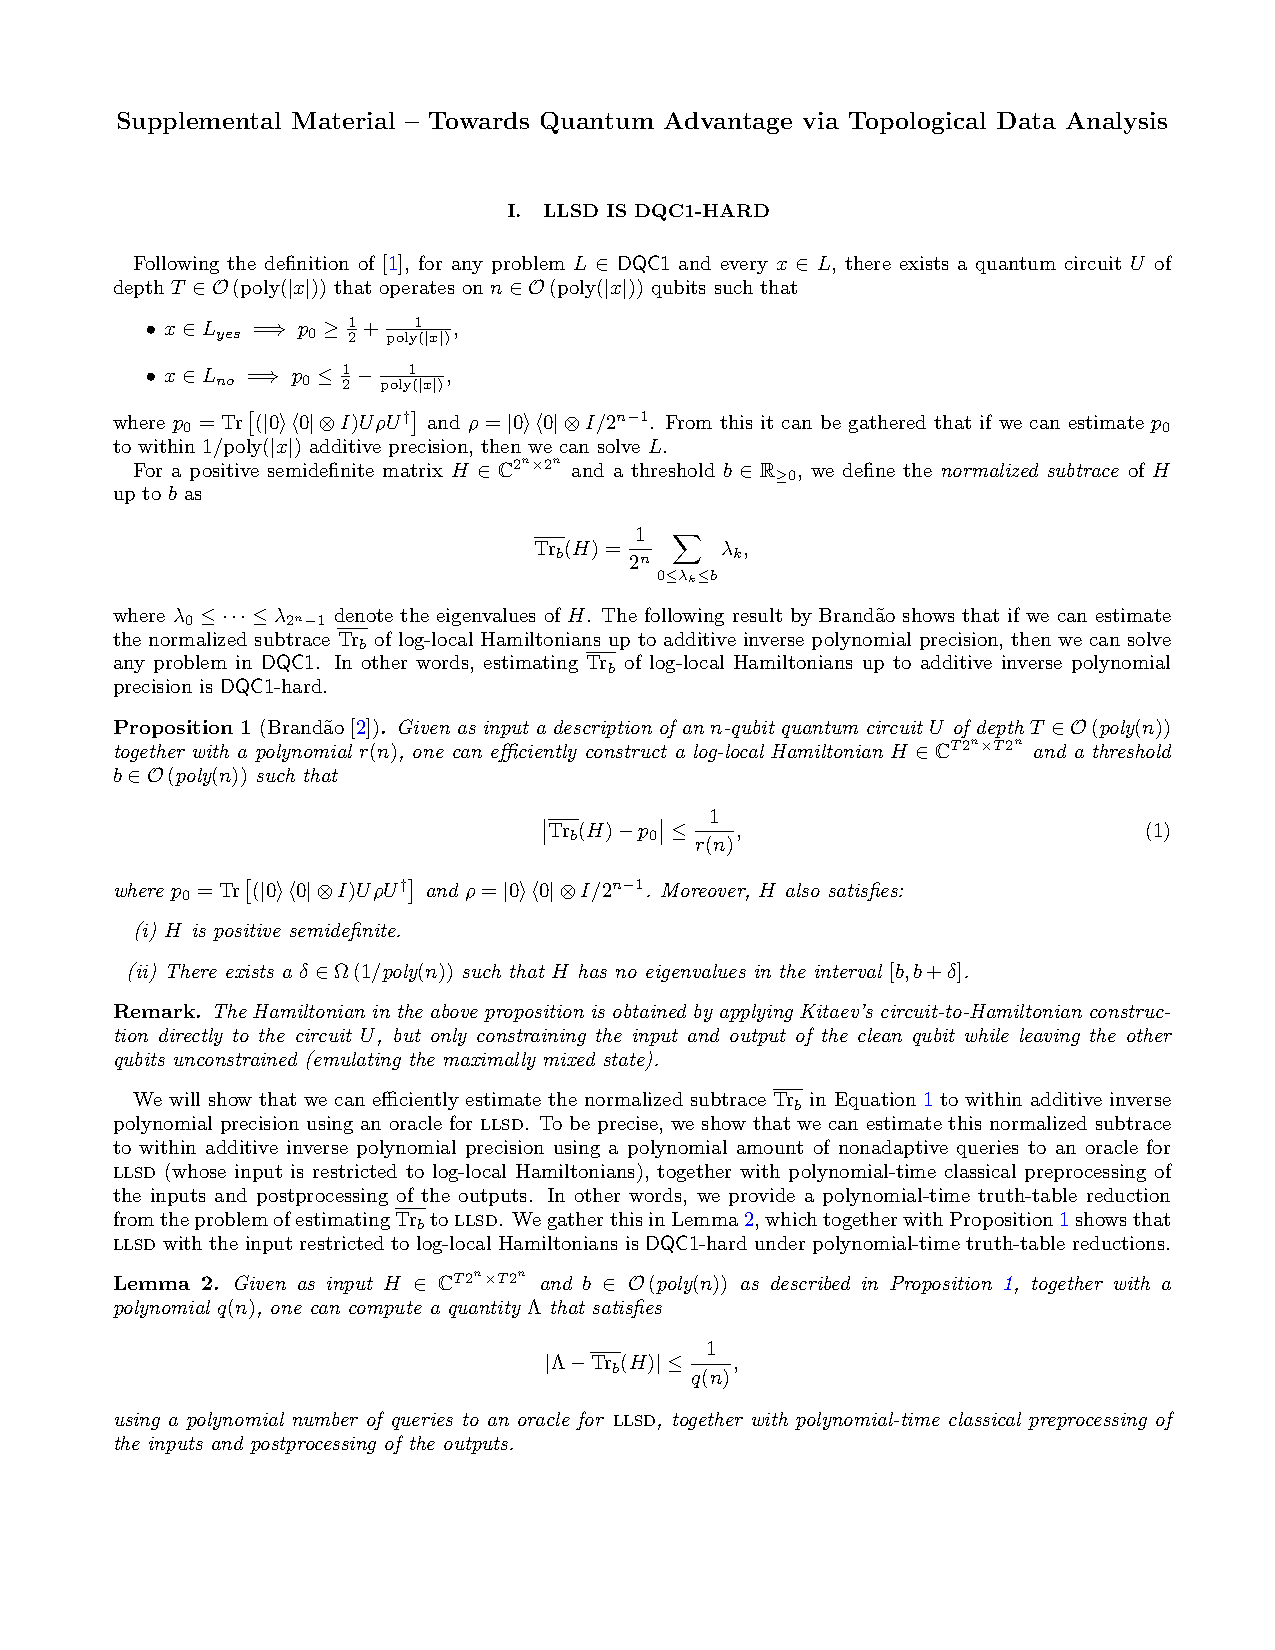
\includepdf[pages={1,2, 3, 4, 5, 6, 7}]{supp.pdf}
%\import{supplemental-material/}{supp}

\end{document}

